\documentclass[11pt,a4paper]{article}

% ── Packages ──
\usepackage[T1]{fontenc}
\usepackage[utf8]{inputenc}
\usepackage{lmodern}
\usepackage[margin=1in]{geometry}
\usepackage{graphicx}
\usepackage{xcolor}
\usepackage{amsmath}
\usepackage{amssymb}
\usepackage{booktabs}
\usepackage{tabularx}
\usepackage{enumitem}
\usepackage{longtable}
\usepackage{fancyhdr}
\usepackage{titlesec}
\usepackage{listings}
\usepackage{needspace}
\usepackage{hyperref}

% ── Hyperref ──
\hypersetup{
    colorlinks=true,
    linkcolor=blue!60!black,
    citecolor=blue!50!black,
    urlcolor=blue!70!black,
    bookmarks=true,
    bookmarksnumbered=true,
    pdftitle={Didactic Manual: big.bi -> bi.gbi Articulatory Simulation},
    pdfauthor={Super Z},
    pdfsubject={Reproduction of arXiv:2307.02299 demonstrations},
    pdfkeywords={articulatory synthesis, syllabification, Maeda model, VLAM, verbal transformation}
}

% ── Page style ──
\pagestyle{fancy}
\fancyhf{}
\fancyhead[L]{\small\itshape big.bi $\to$ bi.gbi --- Didactic Manual}
\fancyhead[R]{\small v1.0}
\fancyfoot[C]{\thepage}
\renewcommand{\headrulewidth}{0.3pt}
\renewcommand{\footrulewidth}{0pt}

% ── Section formatting ──
\titleformat{\section}{\Large\bfseries\color{blue!50!black}}{\thesection}{0.6em}{}
\titleformat{\subsection}{\large\bfseries\color{blue!40!black}}{\thesubsection}{0.5em}{}
\titleformat{\subsubsection}{\normalsize\bfseries}{\thesubsubsection}{0.4em}{}

% ── Listings ──
\definecolor{codebg}{HTML}{F5F5F5}
\definecolor{codeframe}{HTML}{CCCCCC}
\definecolor{codecomment}{HTML}{6A737D}
\definecolor{codekeyword}{HTML}{D73A49}
\definecolor{codestring}{HTML}{032F62}
\lstdefinestyle{pythonstyle}{
    backgroundcolor=\color{codebg}, frame=single,
    rulecolor=\color{codeframe},
    basicstyle=\ttfamily\footnotesize,
    commentstyle=\color{codecomment}\itshape,
    keywordstyle=\color{codekeyword}\bfseries,
    stringstyle=\color{codestring},
    showstringspaces=false, breaklines=true, breakatwhitespace=true,
    numbers=none, xleftmargin=4pt, xrightmargin=4pt,
    framexleftmargin=4pt, framexrightmargin=4pt,
    language=Python,
    morekeywords={panphon_pipeline, vlam, synthSYL, polar_arc, stationary_point}
}
\lstset{style=pythonstyle}

% ── Paragraph spacing ──
\setlength{\parindent}{0pt}
\setlength{\parskip}{0.45em}

\begin{document}

% ════════════════════════════════════════════════════════════════
% Title page
% ════════════════════════════════════════════════════════════════
\begin{titlepage}
\centering
\vspace*{2cm}
{\Huge\bfseries\color{blue!50!black}
Didactic Manual\\[0.3em]
\large big.bi $\to$ bi.gbi\\[0.5em]
\normalsize Articulatory Simulation of the Verbal Transformation
\par}
\vspace{1.5cm}

{\large
Reproduction of the demonstrations described in\\[0.3em]
\textit{``Why can big.bi be changed to bi.gbi?\\
A mathematical model of syllabification and articulatory synthesis''}\\[0.3em]
arXiv:2307.02299 (Berthommier, July 2023)
\par}

\vspace{2cm}

\begin{tabular}{rl}
\textbf{Model:} & VLAM (Maeda, 7 parameters) \\
\textbf{Code:} & Python 3.9+ (MIT License) \\
\textbf{Dependencies:} & numpy, scipy, matplotlib, opencv-python \\
\textbf{Repository:} & \texttt{bigbi-article-repo} \\
\end{tabular}

\vfill

{\small\itshape
This manual provides step-by-step instructions for reproducing the
verbal transformation simulations, including the polar trajectory
visualization, the U-shaped Tp variation, and the comparison with
the article's Figure~4.
}

\vspace{1cm}
{\small Version 1.0 --- \today}
\end{titlepage}

% ════════════════════════════════════════════════════════════════
% Table of contents
% ════════════════════════════════════════════════════════════════
\tableofcontents
\newpage

% ════════════════════════════════════════════════════════════════
% Section 1: Introduction
% ════════════════════════════════════════════════════════════════
\section{Introduction}

This manual documents the Python implementation of the articulatory
speech synthesis model described in arXiv:2307.02299
\cite{berthommier2023}. The model, based on VLAM (a Maeda
articulatory synthesizer with 7 parameters), simulates the
\textbf{verbal transformation} from \texttt{big.bi} to \texttt{bi.gbi}
--- a phenomenon where the syllable boundary shifts as the pause
between syllables is shortened and the anchoring vowels (Vo, Ve)
approach the main vowel V.

The article's central claim (\S4) is:
\begin{quote}
\itshape
``When $\delta_o = \delta_e$ tends to 1 the graph reorganization
can occur because two successive superimposed segments of duration
$2 \times 2T$ anchored to the same vowel $V_o = V_e = V$ can fuse
into a single one of duration $3T$.''
\end{quote}

This repository provides the code to reproduce this transformation
step by step, with audio synthesis, polar trajectory visualization,
and accessible video output.

\subsection{What this repository provides}

\begin{enumerate}[leftmargin=1.4em]
\item The \texttt{synthSYL} package (modified from
\href{https://github.com/FBerthommier/timit-to-Maeda}{FBerthommier/timit-to-Maeda})
with the $\delta_o$ and $\delta_e$ parameters added to
\texttt{panphon\_pipeline()}.

\item The VLAM synthesizer (\texttt{vlam.py}) for audio generation
from Maeda parameters.

\item Simulation scripts for three demonstrations:
  \begin{itemize}
  \item \texttt{big.bi $\to$ bi.gbi} (the article's main result, \S4)
  \item \texttt{ib ib $\to$ bi bi} (the classical transformation, \S3)
  \item U-shaped $T_p$ variation for perceptual demonstration
  \end{itemize}

\item Polar trajectory reconstruction (two-branch: vocalic $z_v$
and consonantal $z_c$), using primitives from
\href{https://github.com/FBerthommier/covtl-pipeline}{FBerthommier/covtl-pipeline}.

\item Dual-panel video generation (sagittal vocal tract | polar plot)
with synchronized audio and phoneme labels.
\end{enumerate}

\subsection{The VLAM model}

VLAM (Vocal tract Learner Articulatory Model) is the Maeda model
with 7 articulatory parameters:
\begin{center}
\begin{tabular}{cll}
\toprule
\textbf{Index} & \textbf{Symbol} & \textbf{Description} \\
\midrule
0 & J  & Jaw opening \\
1 & B  & Tongue body position \\
2 & D  & Tongue dorsum height \\
3 & T  & Tongue tip position \\
4 & LP & Lip protrusion/rounding \\
5 & LH & Vertical lip opening \\
6 & Hy & Larynx height \\
\bottomrule
\end{tabular}
\end{center}

\textbf{Indexing convention.} Two numbering conventions coexist and
must not be mixed:
\begin{itemize}
\item the \textbf{article} numbers the parameters $1$--$7$
  ($1$=Jaw, $2$=Body, $3$=Dorsum, $4$=Tip, $5$=LipP, $6$=LipH,
  $7$=Hy); its selection vectors $S_c$ and $S_v$ (e.g.\
  $S_c = \{1,2,6\}$) use this 1-based numbering;
\item the \textbf{code} (and the table above) numbers them $0$--$6$;
  the registry selection vectors are 0-based, e.g.\ /b/ has
  \texttt{params=[0,1,5]}.
\end{itemize}
Correspondence: article $\{1,2,6\}$ = code $\{0,1,5\}$ = \{Jaw, Body,
LipH\}; article $\{1,2,3,4\}$ = code $\{0,1,2,3\}$ = \{Jaw, Body,
Dorsum, Tip\}; article $S_v = \{3,4,5,7\}$ = code $\{2,3,4,6\}$ =
\{Dorsum, Tip, LipP, Hy\}. Throughout this manual, $S_c$/$S_v$ sets
are quoted in the article's 1-based numbering (as in the article),
while parameter indices mentioned in the text refer to the 0-based
code indices unless stated otherwise.

The coordination function (article Eq.~1) maps a polar target
$(\rho, \theta)$ to the 7 Maeda parameters:
\begin{equation}
P_i = \Omega_i + \rho \cdot \Psi_{1,i} \cdot \cos(\Psi_{2,i} - \theta)
\label{eq:coordination}
\end{equation}

where $\Omega$, $\Psi_1$, and $\Psi_2$ are calibration constants
(article Table~1). The CO matrix in \texttt{synthSYL/constants.py}
matches the article's Table~1 almost exactly (only the Tip parameter
$c_0$ differs slightly: $-2.75$ in synthSYL vs $-3.0$ in the article).

\subsection{Article parameters}

The article (\S2.1) specifies the following arc parameters:
\begin{itemize}
\item $K_{\text{voy}} = 30$ --- vowel arc curvature
\item $K = 10$ --- consonant arc curvature
\item $P_{\text{exp}} = 1$ --- velocity profile exponent
  ($\rho(t) = \cos(\theta(t)/2)$, not $\cos^2$)
\item $T = 16$ --- time step (didactic mode)
\item $\nu = -1$ --- coarticulation index
\end{itemize}

These are set in \texttt{synthSYL/constants.py}:
\begin{lstlisting}
DEFAULT_T: int = 16
DEFAULT_K: int = 10        # consonant arc curvature
DEFAULT_KVOY: int = 30     # vowel arc curvature
DEFAULT_PEXP: int = 1      # velocity profile exponent
DEFAULT_NU: int = -1
\end{lstlisting}

The article notes: \textit{``When $K$ is large ($K = 30$ for vowel
arcs and $K = 10$ for consonant arcs), the trajectories become
straight lines.''} With $P_{\text{exp}} = 1$, the velocity profile
follows $\cos(\theta/2)$ (a cosine half-bell) rather than
$\cos^2(\theta/2)$ (a Hanning window).

\textbf{Note on display curvature:} The polar trajectory
visualization uses $K = 30$ for both vocalic and consonantal branches
(the covtl-pipeline reference display curvature), not the engine's
$K = 10$ / $K_{\text{voy}} = 30$. This is a deliberate visualization
choice that produces moderate, visible curvature for both branches.

% ════════════════════════════════════════════════════════════════
% Section 2: The Mathematical Model
% ════════════════════════════════════════════════════════════════
\section{The Mathematical Model}

\subsection{Polar coordinates and targets}

Each phoneme target is a point $(\rho, \theta)$ in the complex
plane:
\begin{itemize}
\item \textbf{Vowels}: $\rho \in [0, 1]$, $\theta \in [0, 2\pi)$
\item \textbf{Consonants}: $\rho \in [0, 1.2]$, $\theta \in [0, 2\pi)$
\end{itemize}

For example, the vowel /i/ is at $(\rho=0.9, \theta=5\pi/3)$ and the
consonant /b/ is at $(\rho=1.2, \theta=\pi/3)$.

\subsection{Arc trajectories}

Motion between two targets $(\rho_1, \theta_1)$ and
$(\rho_2, \theta_2)$ is produced by the arc function (article Eq.~2):
\begin{equation}
z(t) = (1 - r_k) \cdot \rho_1 e^{i\theta_1}
     + r_k \cdot \rho_2 \cdot e^{i(\theta_2 + \frac{\nu}{K} \cdot \text{th})}
\label{eq:arc}
\end{equation}

where $r_k = \cos^{P_{\text{exp}}}(\text{th}/2)$ is the velocity profile,
$\text{th} \in [0, \pi]$ is a half-turn sweep, $\nu = \pm 1$
controls the curvature direction, and $K$ is the curvature constant
($K=30$ for display, $K=10$ for consonant arcs, $K_{\text{voy}}=30$
for vowel arcs in the synthesis engine).

\textbf{Important:} The article uses $P_{\text{exp}} = 1$, so
$r_k = \cos(\text{th}/2)$ (a cosine half-bell, \textit{without} the
power of 2). This is the form used for all demonstrations in this
repository. The original \texttt{synthSYL} package used $P_{\text{exp}}
= 2$ ($r_k = \cos^2(\text{th}/2)$, a Hanning window), which has been
corrected to match the article.

\subsection{Anchoring vowels: Vo and Ve}

The article (\S2.2) introduces two anchoring vowels:
\begin{align}
V_o &= (\delta_o \cdot \rho_V, \theta_V) \\
V_e &= (\delta_e \cdot \rho_V, \theta_V)
\end{align}

\begin{itemize}
\item $V_o$ (onset): anticipation of the vowel before the consonant.
  The value of $\delta_o$ determines the degree of anticipation.
\item $V_e$ (end): centralization of the coda vowel (schwa-like
  vocoid). Modeled with $\delta_e = 0.5$ (salient) or $\delta_e = 0.7$
  (audible).
\end{itemize}

When $\delta_o = \delta_e \to 1$, both $V_o$ and $V_e$ approach $V$
(the full vowel), enabling the fusion of adjacent syllable segments.

\subsection{Superposition}

The final parameter frame is a blend (article Eq.~4):
\begin{equation}
\tag{art.\,4}
P(t) - \Omega = \text{Re}\left[ S_v \cdot \Psi \cdot \bar{z}_v(t)
                              + S_c \cdot \Psi \cdot \bar{z}_c(t) \right]
\end{equation}

where $S_v$ and $S_c$ are selection vectors (binary masks over the
7 parameters), $z_v(t)$ is the vocalic trajectory, and $z_c(t)$ is
the consonantal trajectory.

% ════════════════════════════════════════════════════════════════
% Section 3: The Syllable Graph Architecture
% ════════════════════════════════════════════════════════════════
\section{The Syllable Graph Architecture}

\subsection{CV graph}

A CV syllable (e.g., /bi/) has 3 nodes and 4 arcs:
\begin{itemize}
\item Nodes: $V = \{V_o, C, V\}$
\item Locations: $L = \{(\delta_o \rho_V, \theta_V),\;
  (\rho_C, \theta_C),\;(\rho_V, \theta_V)\}$
\item Arcs: $E = \{(V_o, C), (C, V), (V_e, V), (V, V)\}$
\item Durations: $T_p = \{T_1, T_2, 2T_2, T\}$
\end{itemize}

\subsection{CVC graph}

A CVC syllable (e.g., /big/) has 5 nodes, symmetric with respect to
the CV graph:
\begin{itemize}
\item Nodes: $V = \{V_o, C_1, V, C_2, V_e\}$
\item Locations: $L = \{(\delta_o \rho_V, \theta_V),\;
  (\rho_{C_1}, \theta_{C_1}),\;(\rho_V, \theta_V),\;
  (\rho_{C_2}, \theta_{C_2}),\;(\delta_e \rho_V, \theta_V)\}$
\end{itemize}

\subsection{CCV graph (clusters)}

A CCV syllable (e.g., /gbi/) has 4 nodes and 5 arcs:
\begin{itemize}
\item Nodes: $V = \{V_o, C_1, C_2, V\}$
\item Arcs: $E = \{(V_o, C_1), (C_1, C_2), (C_2, V), (V_e, V), (V, V)\}$
\item The consonantal branch visits $C_1$ then $C_2$ in sequence.
\end{itemize}

\subsection{The fusion mechanism}

The article (\S4) describes the fusion:
\begin{quote}
\itshape
``When $\delta_o = \delta_e$ tends to 1 the graph reorganization
can occur because two successive superimposed segments of duration
$2 \times 2T$ anchored to the same vowel $V_o = V_e = V$ can fuse
into a single one of duration $3T$.''
\end{quote}

The gain is twofold:
\begin{enumerate}
\item \textbf{Consonant clustering}: reduction of one period $T$
  (from 2 separate consonant gestures to 1 fused cluster gesture).
\item \textbf{Node loss}: the $V$ node between the two syllables
  disappears (since $V_o = V_e = V$), reducing the graph complexity.
\end{enumerate}

Additionally, the selection vector switches (article's 1-based
numbering; code indices subtract 1):
\begin{itemize}
\item Before fusion: $S_c = \{1,2,3,4\}$ for /g/ and $S_c = \{1,2,6\}$
  for /b/ (two separate gestures)
\item After fusion: $S_c = \{1,2,3,6\}$ for /gb/ (one fused gesture)
\end{itemize}

% ════════════════════════════════════════════════════════════════
% Section 4: The delta parameters
% ════════════════════════════════════════════════════════════════
\section{The $\delta_o$ and $\delta_e$ Parameters}

\subsection{Implementation}

The $\delta_o$ and $\delta_e$ parameters are added to the
\texttt{panphon\_pipeline()} function as optional keyword arguments:

\begin{lstlisting}
from synthSYL import panphon_pipeline

result = panphon_pipeline(
    "big bi",
    T=16,
    short_pause_duration_factor=1.0,
    delta_o=0.5,   # Vo = (0.5 * rho_V, theta_V)
    delta_e=0.5,   # Ve = (0.5 * rho_V, theta_V)
)
\end{lstlisting}

The default values are $\delta_o = \delta_e = \texttt{COEFCEN} = 0.5$,
preserving backward compatibility with the original package.

\subsection{Effect on the anchoring vowels}

Table~\ref{tab:delta} shows the effect of $\delta$ on the anchoring
vowels for the vowel /i/ ($\rho_V = 0.9$, $\theta_V = 5\pi/3$):

\begin{table}[h]
\centering
\caption{Effect of $\delta$ on $V_o$ and $V_e$ (for /i/)}
\label{tab:delta}
\begin{tabular}{cccc}
\toprule
$\delta$ & $V_o = V_e$ $\rho$ & Perception & Article term \\
\midrule
0.50 & 0.450 & Salient schwa @ & ``salient'' \\
0.70 & 0.630 & Audible schwa   & ``audible'' \\
0.85 & 0.765 & Residual schwa  & --- \\
0.95 & 0.855 & $V_o \approx V_e \approx V$ & --- \\
1.00 & 0.900 & $V_o = V_e = V$ (fusion) & --- \\
\bottomrule
\end{tabular}
\end{table}

\subsection{The $V_e$ plateau --- revoked}

An earlier revision of this repository added a full-amplitude
$V_e$ plateau before the decay block (\texttt{trajectory.py},
\texttt{\_handle\_b\_terminal()}), reasoning that ``$V_e$ is a NODE''
(\S2.2) and should therefore be held like $V$. This addition has been
\textbf{revoked} (author ruling 2026-10-07): a reduced word-end vowel
is not pronounced as a tensed vowel --- one does not pronounce
``ibe'' --- so there is NO held @. The engine now behaves like the
reference \texttt{timit-to-Maeda}: the trajectory \emph{reaches} the
$V_e$ anchor and decays immediately, with no extra hold. The
reference \texttt{\_handle\_b\_terminal()} chains the decay directly:

\begin{lstlisting}
elif A.kind == "V":
    if B.kind == "pause":
        pt_A = _safe_pt(A)
        _append_decay_block(blocks, block_info, pt_A, T_cons, pre_amp=1.0)
\end{lstlisting}

Our engine now matches this (the final vowel of a CV word is still
held through the regular last-anchor hold; only the extra pre-decay
$V_e$ plateau is gone). All reference reproductions remain
bit-identical ($0.000e+00$): /ibia/ never had a $V_e$ plateau, and
the words whose acoustics change (e.g.\ /ib/) are not part of the
stored reference gates.

% ════════════════════════════════════════════════════════════════
% Section 5: Reproduction Guide
% ════════════════════════════════════════════════════════════════
\section{Reproduction Guide}

\subsection{Installation}

\begin{lstlisting}[language=bash]
# Clone the repository
git clone https://github.com/<your-org>/bigbi-article-repo.git
cd bigbi-article-repo

# Install Python dependencies
pip install -r requirements.txt

# (Optional) Install ffmpeg for video generation
sudo apt install ffmpeg  # Linux
# brew install ffmpeg     # macOS
\end{lstlisting}

\subsection{Demonstration 1: big.bi $\to$ bi.gbi (Article \S4)}

This is the main demonstration, showing the verbal transformation
with $T=16$ (didactic mode), starting at $\delta = 0.50$ for a
salient boundary schwa @. \textbf{Dot form} (author ruling
2026-10-07): big.bi is synthesized as the dotted word
\texttt{big.bi} --- the '.' between /g/ and /b/ is a C.C syllable
boundary with \emph{no pause} (the reference Timit-to-Maeda
semantics: the Ve of ``big'' is coarticulated with the /i/ of
``bi'', the boundary anchor weighted by COEFCEN). There is therefore
\emph{no} $T_p$/pause dimension in this sweep: $\delta$ alone drives
the transformation (boundary anchor $= \delta \cdot \rho_i$; at
$\delta = 1$ the anchor is the full /i/, fusion-ready).

\begin{lstlisting}[language=bash]
# Run the sweep (14 segments: 11 "big.bi" + 3 "bi.gbi")
python scripts/run_bigbi_polar_sweep.py

# Generate the dual-panel video (sagittal | polar)
python scripts/make_bigbi_dual_video.py

# Generate the self-contained HTML with embedded video
python scripts/embed_video_in_html.py en
\end{lstlisting}

The output is in \texttt{output/bigbi\_polar\_sweep/}:
\begin{itemize}
\item \texttt{dual/dual\_progressive.mp4} --- dual-panel video
  ($\approx$ 24.2~s, 1.4~MB)
\item \texttt{polar/polar\_progressive.mp4} --- polar-only video (3.3~MB)
\item \texttt{index\_embedded.html} --- self-contained HTML
  (re-embedded in \texttt{simulations/})
\end{itemize}

\subsection{Demonstration 2: U-shaped $T_p$ variation}

The U-shaped variation lets the listener clearly perceive:
\texttt{ib ib} at the start $\to$ \texttt{bi bi} at the bottom
(fusion) $\to$ \texttt{ib ib} again at the end. This $T_p$ sweep is
the /ibi/ supplement demonstration (\S3 classical transformation),
where the inter-word pause IS the object of study; it is distinct
from the big.bi sweep of Demonstration~1, which — in the dot form —
carries no $T_p$ dimension.

\begin{lstlisting}[language=bash]
python scripts/run_ibbi_ushape_sweep.py
\end{lstlisting}

The sweep is a \textbf{continuous U-shaped ramp} of \textbf{10
segments}: $T_p$ decreases to 0 with $\delta$ correlated at every
point ($\delta = 0.5 + 0.5\,(1 - T_p/160)$), then increases back to
the 160-ms baseline; consecutive segments flow directly into one
another (no restarts):
\begin{center}
\begin{tabular}{lccc}
\toprule
 & Segments & $T_p$ (ms) & $\delta$ \\
\midrule
descent & 1--4 & 160, 120, 80, 40 & 0.50 \dots 0.875 \\
bottom (fusion, \texttt{bi bi}) & 5 & 0 & \textbf{1.000} \\
ascent & 6--9 & 40, 80, 120, 160 & 0.875 \dots 0.50 \\
end baseline & 10 & 160 & 0.500 \\
\bottomrule
\end{tabular}
\end{center}
Duration $\approx$ 18.6~s. Note: the coda @ is \emph{not} held --- the
trajectory reaches the word-end anchor and decays immediately (no
``ibe'').

\subsection{Demonstration 3: Comparison with the article}

To compare our polar figures with the article's Figure~4:

\begin{lstlisting}[language=bash]
# Generate the comparison figure
python scripts/compare_article_polar.py
\end{lstlisting}

This produces a 2$\times$2 grid: article Figure~4 (top) vs our
simulation (bottom), for both \texttt{big.bi} ($\delta=1$) and
\texttt{bi.gbi}.

% ════════════════════════════════════════════════════════════════
% Section 6: Polar Trajectory Reconstruction
% ════════════════════════════════════════════════════════════════
\section{Polar Trajectory Reconstruction}

The two-branch polar visualization (vocalic $z_v$ in red,
consonantal $z_c$ in blue) is rebuilt from the engine's
\textbf{recorded block sequence} by \texttt{scripts/polar\_sync.py}
(\texttt{record\_pipeline} instruments the trajectory helpers without
touching the engine files; \texttt{build\_branches} then draws both
branches from the blocks the engine actually walked). The original
\texttt{Syllable\_Synthesis} display anchoring is used --- see
\texttt{docs/DISPLAY\_VS\_ENGINE.md} for the full audit:

\begin{itemize}
\item every sub-arc carries the phase on the \textbf{arrival-side}
  point ($p_a$) with the departure-side point $p_d$ held fixed ($p_d$
  = the consonant on $z_c$ approach legs, $V_1$ on vocalic
  backgrounds) --- this is the reference convention, not an option;
\item the approach leg sweeps $\theta \in [0, \pi]$ (opint $= 0$),
  the release legs and vocalic backgrounds $\theta \in [-\pi, 0]$
  (opint $= -1$, first sample dropped, for the releases);
\item $\rho = \cos(\theta/2)$ ($P_{\exp} = 1$).
\end{itemize}

\subsection{Reconstruction rules}

\begin{center}
\begin{tabularx}{\textwidth}{@{}>{\raggedright\arraybackslash}p{0.26\textwidth}X@{}}
\toprule
\textbf{Block kind} & \textbf{Branch behavior} \\
\midrule
plateau, attack, decay & red: stationary anchor; blue: inactive \\
background, pause & red: arcplot arc $(V_1 \to V_2)$ with $K=30$,
                  $\nu_v = -1$; blue: inactive \\
cluster ($n = (m{+}1)T$ steps) & red: arcplot arc $(V_1 \to V_2)$ over
                  the whole block; blue: sub-arcs $V_1 \to C_1 \to
                  \dots \to C_m \to V_e$, $T$ steps each, $K=10$,
                  $\nu_c = +1$, approach leg $[0, \pi]$ then release
                  legs $[-\pi, 0]$ --- the closed V$\to$C$\to$V
                  gesture is a \textbf{teardrop} (belly at the vowel,
                  point at the consonant), as in the article's
                  Figure~4 \\
\bottomrule
\end{tabularx}
\end{center}

\subsection{Display curvature and $\nu$ convention}

The display uses the article values $K = 30$ for $z_v$ and $K = 10$
for $z_c$ (\S2.1), and the per-branch display convention
$\nu_v = -1$, $\nu_c = +1$ (the article's planning-figure convention;
the engine itself drives every arc with the single value $\nu = -1$).
The legacy \texttt{polar\_arc} form for $z_v$ (mirrored phase sweep)
remains available as \texttt{zv\_form="polar\_arc"} for the record.

\subsection{Comparison with the article's Figure~4}

Under the article figure conditions (COEFCEN $= 1$, VOYDEB $= 0.5$,
$T = 16$), the reproduced planning panels
(\texttt{docs/figures/article\_format/figure4\_bigbi\_bigbi.png},
\texttt{fig\_bigbi\_article\_conditions\_nu\_inv.png} and
\texttt{fig\_words\_article\_conditions\_nu\_inv.png}) show:
\begin{itemize}
\item big.bi: \textbf{3} separate $z_c$ gestures --- /b/ (onset),
  palatal /g/ (coda), /b/ (word-2 onset, a closed loop anchored on
  the previous $V_e$);
\item bi.gbi: \textbf{2} gestures --- /b/ + the fused /gb/ cluster
  (single span visiting /g/ then /b/);
\item the red $z_v$ branch: schwa loop at the word onset
  ($V_o$ at half radius), full vowel elsewhere ($V_e = V$ under
  COEFCEN $= 1$).
\end{itemize}

The article's Figure~4 uses a different polar target table (the
AP-model layout; see \texttt{docs/TRAJECTORY\_MATCHING.md}), so the
panel-level comparison is gestural (same teardrop topology, same
gesture counts), not a point-wise overlay.

% ════════════════════════════════════════════════════════════════
% Section 7: Results and Duration Analysis
% ════════════════════════════════════════════════════════════════
\section{Results and Duration Analysis}

\subsection{Duration reduction}

The article predicts a duration reduction when transitioning from
\texttt{big.bi} ($\delta < 1$) to \texttt{bi.gbi} ($\delta = 1$):

\begin{quote}
\itshape
``At first, the gain of consonant clustering is a reduction of one
period $T$. The graph complexity is corollary reduced with a decay
of the number of nodes with the loss of $V$.''
\end{quote}

With $T=16$, in the dot form (no pause --- the block layout does not
depend on $\delta$, only the anchor values do), our simulation shows:

\begin{center}
\begin{tabular}{lcccc}
\toprule
\textbf{Configuration} & $\delta$ & Steps & Duration (ms) & Reduction \\
\midrule
big.bi (dot, start) & 0.50 & 176 & 1760 & --- \\
big.bi (dot, pre-fusion) & 0.995 & 176 & 1760 & --- \\
bi.gbi (fused) & 1.00 & 160 & 1600 & $-160$ ms ($-1T$) \\
\bottomrule
\end{tabular}
\end{center}

The observable fusion gain is $1T = 160$~ms, from consonant
clustering: the fused /gb/ cluster chains the /g/$\to$/b/ sub-arcs
directly through the shared vowel anchor, and the separate syllable-2
onset gesture disappears. (The earlier $\approx 3T$ reading compared
against the space form ``big bi'' included the inter-word pause
machinery --- decay + pause arc $\approx 2T$ --- which, as established,
is not part of big.bi: the '.' is a C.C syllable boundary without
pause, and the only latencies are the stop closures.)

\subsection{Audio verification: per-segment WAVs, /i/ height, valrect}

Every simulation writes its segments as SEPARATE WAV files, so the
/i/ vowels can be compared by ear:
\begin{itemize}
\item \texttt{output/ibbi\_ushape\_en/wav/synth\_sNN\_tpXXX.wav} ---
  reversible U-shape, one file per segment;
\item \texttt{output/ibbi\_ushape\_nonrev\_en/wav/} --- non-reversible;
\item \texttt{output/bigbi\_polar\_sweep/wav/synth\_dXXX.wav} ---
  big.bi $\to$ bi.gbi sweep;
\item \texttt{output/article\_demos/} and
  \texttt{output/trough\_ablations/} --- article reproductions and
  trough-effect measurements.
\end{itemize}

Measured on the current 10-segment sweeps (autocorrelation F0 on the
vowel plateaus): the median F0 is constant across segments
($\approx$ 119--124~Hz, cf0 $= 1.0$ everywhere) --- the /i/ vowels all
sit at the same pitch; the small median shift between ``ib ib'' and
``bi bi'' segments is a formant-related measurement bias, not a pitch
difference. No digital clipping anywhere ($<$0.02\,\% of samples at
peak). \texttt{valrect} (the soft-rectification smoothness of the
vocal-tract area function, \texttt{soft\_rect(x, s)} with
$s = 0$ $\equiv$ hard rectification) is \textbf{1.10 in every
script} (author ruling 2026-10-07: raised from the article's
canonical 0.75 after comparative listening, to reduce the perceived
fizz on /i/; see \texttt{docs/VALRECT\_110.md} for the re-baselined
reference). Measured on ``bi bi''/``ib ib'' test utterances, the
high-frequency energy ratio above 5~kHz decreases from 0.17\,\% to
0.15\,\% (``bi bi'') and from 0.13\,\% to 0.12\,\% (``ib ib'')
between 0.75 and 1.10, with no change in F0 or duration; test WAVs
for listening comparison are kept outside the repository
(\texttt{P:$\backslash$bigbi-workspace$\backslash$valrect\_test\_*.wav}).

\subsection{Perceptual salience of the schwa @}

With $T=16$ and $\delta = 0.50$, the boundary schwa @ in
\texttt{big.bi} is \textbf{salient} (clearly perceivable) because:
\begin{enumerate}
\item the C.C boundary anchor sits at $\rho = 0.45$ (most
  centralized, far from the full vowel /i/ at $\rho = 0.9$);
\item the $z_v$ background dips to that anchor between the /g/ and
  /b/ clusters (audible schwa-like vocoid);
\item there is no pause: the schwa is carried by the planning
  trajectory through the consonant--consonant chain, exactly as the
  dot semantics prescribe.
\end{enumerate}

As $\delta$ increases toward 1.0, the boundary anchor approaches
$V = /i/$ (COEFCEN $= 1$) and the perception shifts from
\texttt{big.bi} to \texttt{bi.gbi}.

% ════════════════════════════════════════════════════════════════
% Section 8: Code Structure
% ════════════════════════════════════════════════════════════════
\section{Code Structure}

\subsection{Modified files (vs original timit-to-Maeda)}

\begin{center}
\begin{tabular}{ll}
\toprule
\textbf{File} & \textbf{Modification} \\
\midrule
\texttt{synthSYL/constants.py} & Added \texttt{DEFAULT\_DELTA\_O},
  \texttt{DEFAULT\_DELTA\_E} \\
\texttt{synthSYL/gesture.py} & Added $\delta_o$, $\delta_e$ kwargs
  to \texttt{build\_gesture\_anchors()}, \\
  & \texttt{\_insert\_word\_end\_anchors()},
  \texttt{\_insert\_vowel\_onset\_anchors()}, \\
  & \texttt{\_insert\_syllable\_onset\_anchors()} \\
  & Fixed $V_o = (\delta_o \cdot \rho_V, \theta_V)$
  (was $[\delta_o, \theta_V]$) \\
\texttt{synthSYL/trajectory.py} & REVOKED addition: the $V_e$ plateau
  (full-amplitude before decay) was added in an earlier revision and
  removed on 2026-10-07 --- the decay now chains directly on the
  word-end anchor (no held @), as in the reference package \\
\texttt{synthSYL/pipeline.py} & Added $\delta_o$, $\delta_e$ kwargs
  to \texttt{panphon\_pipeline()} \\
\bottomrule
\end{tabular}
\end{center}

\subsection{Simulation scripts}

\begin{center}
\begin{tabular}{ll}
\toprule
\textbf{Script} & \textbf{Purpose} \\
\midrule
\texttt{run\_bigbi\_polar\_sweep.py} & Main sweep: big.bi $\to$ bi.gbi
  with polar coords \\
\texttt{run\_ibbi\_ushape\_sweep.py} & U-shaped $T_p$ variation \\
\texttt{make\_bigbi\_dual\_video.py} & Dual-panel video generation \\
\texttt{make\_ibbi\_polar\_video.py} & Polar-only video generation \\
\texttt{make\_article\_figures.py} & Article-format Figures 1/3/4 +
  article-conditions planning panels \\
\texttt{embed\_video\_in\_html.py} & Self-contained HTML (base64 video) \\
\texttt{compare\_article\_polar.py} & Compare with article Figure~4 \\
\bottomrule
\end{tabular}
\end{center}

% ════════════════════════════════════════════════════════════════
% Section 9: Quick Demo
% ════════════════════════════════════════════════════════════════
\section{Quick Demo}

The minimal code to run the big.bi $\to$ bi.gbi simulation:

\begin{lstlisting}
from synthSYL import panphon_pipeline
import vlam
import numpy as np
from scipy.io.wavfile import write

# Run the pipeline for "big bi" at delta=0.5 (salient schwa)
result = panphon_pipeline(
    "big bi",
    T=16,
    short_pause_duration_factor=1.0,
    delta_o=0.5,
    delta_e=0.5,
)

# Synthesize audio
state = vlam.VlamState.initial(195)
config = vlam.SynthConfig(play_audio=False)
sr = vlam.synthwordfen(
    state=state,
    articulatory_params=result.Pval,
    word_tokens=["O", "V", "F"],
    duration_factor=16,
    envelope=result.envelope,
    config=config,
)

# Save WAV
sig = sr.signal
sig_int16 = np.int16(32767 * sig / (1.01 * np.max(np.abs(sig))))
write("big_bi_delta05.wav", 20000, sig_int16)
print(f"Signal: {sig.shape[0]} samples ({sig.shape[0]/20000*1000:.0f} ms)")
\end{lstlisting}

% ════════════════════════════════════════════════════════════════
% Section 11: Article Demonstrations
% ════════════════════════════════════════════════════════════════
\section{Article Demonstrations}

This section documents four additional demonstrations from the article
that have been implemented in this repository: Demo~1 (/ibia/),
Demo~2 (locus equations), Demo~3 (trough effect) and Demo~4
(consonant clusters).

\subsection{Demo 1: /ibia/ VCV synthesis (Figure 1)}

The article's Figure~1 shows the four-step synthesis pipeline on the
sequence /ibia/ (/i/ $\to$ /b/ $\to$ /i/ $\to$ /a/). The four panels
are:

\begin{enumerate}
\item \textbf{(a) Planning trajectories} $z_v(t)$ and $z_c(t)$ in the
  polar plane $(\rho, \theta)$, article format. The vocalic branch
  $z_v$ (red) flows from /i/ to /i/ to /a/, while the consonantal
  branch $z_c$ (blue) makes a teardrop excursion toward the /b/
  target.

\item \textbf{(b) Flow of articulatory parameters} --- the 7 Maeda
  parameters over time. The \textit{Body} parameter makes an
  unexpected front/back movement during /b/, rising toward the /u/
  direction, because /b/ lies on the same angular direction as /u/ in
  the complex plane (see Demo~3). With the synthSYL registry default
  $\rho_b = 1.2$ used by this figure, the Body peaks at $+1.50$
  (measured) above the /i/ plateau $-2.25$; the article position
  $\rho_b = 1.0$ gives $+1.25$.

\item \textbf{(c) Formant trajectory} F1-F2-F3. F2 rises from its
  initial (neutral-onset) value ($\approx 1830$~Hz, measured
  $1826$~Hz at frame~0) to the /i/ plateau ($\approx 2280$~Hz,
  measured $2276$~Hz), dips during /b/ in a V-shaped valley (minimum
  $1570$~Hz at $\rho_b = 1.2$, mid-closure), rises back to the /i/
  level, then falls toward /a/. This is a V-shaped perturbation, not
  an S-shape: the F2 pattern through the consonant is a single
  minimum between two vowel plateaus.

\item \textbf{(d) Output spectrogram + wave} showing the acoustic
  result (waveform superposed on the grayscale spectrogram).
\end{enumerate}

\begin{figure}[h]
\centering
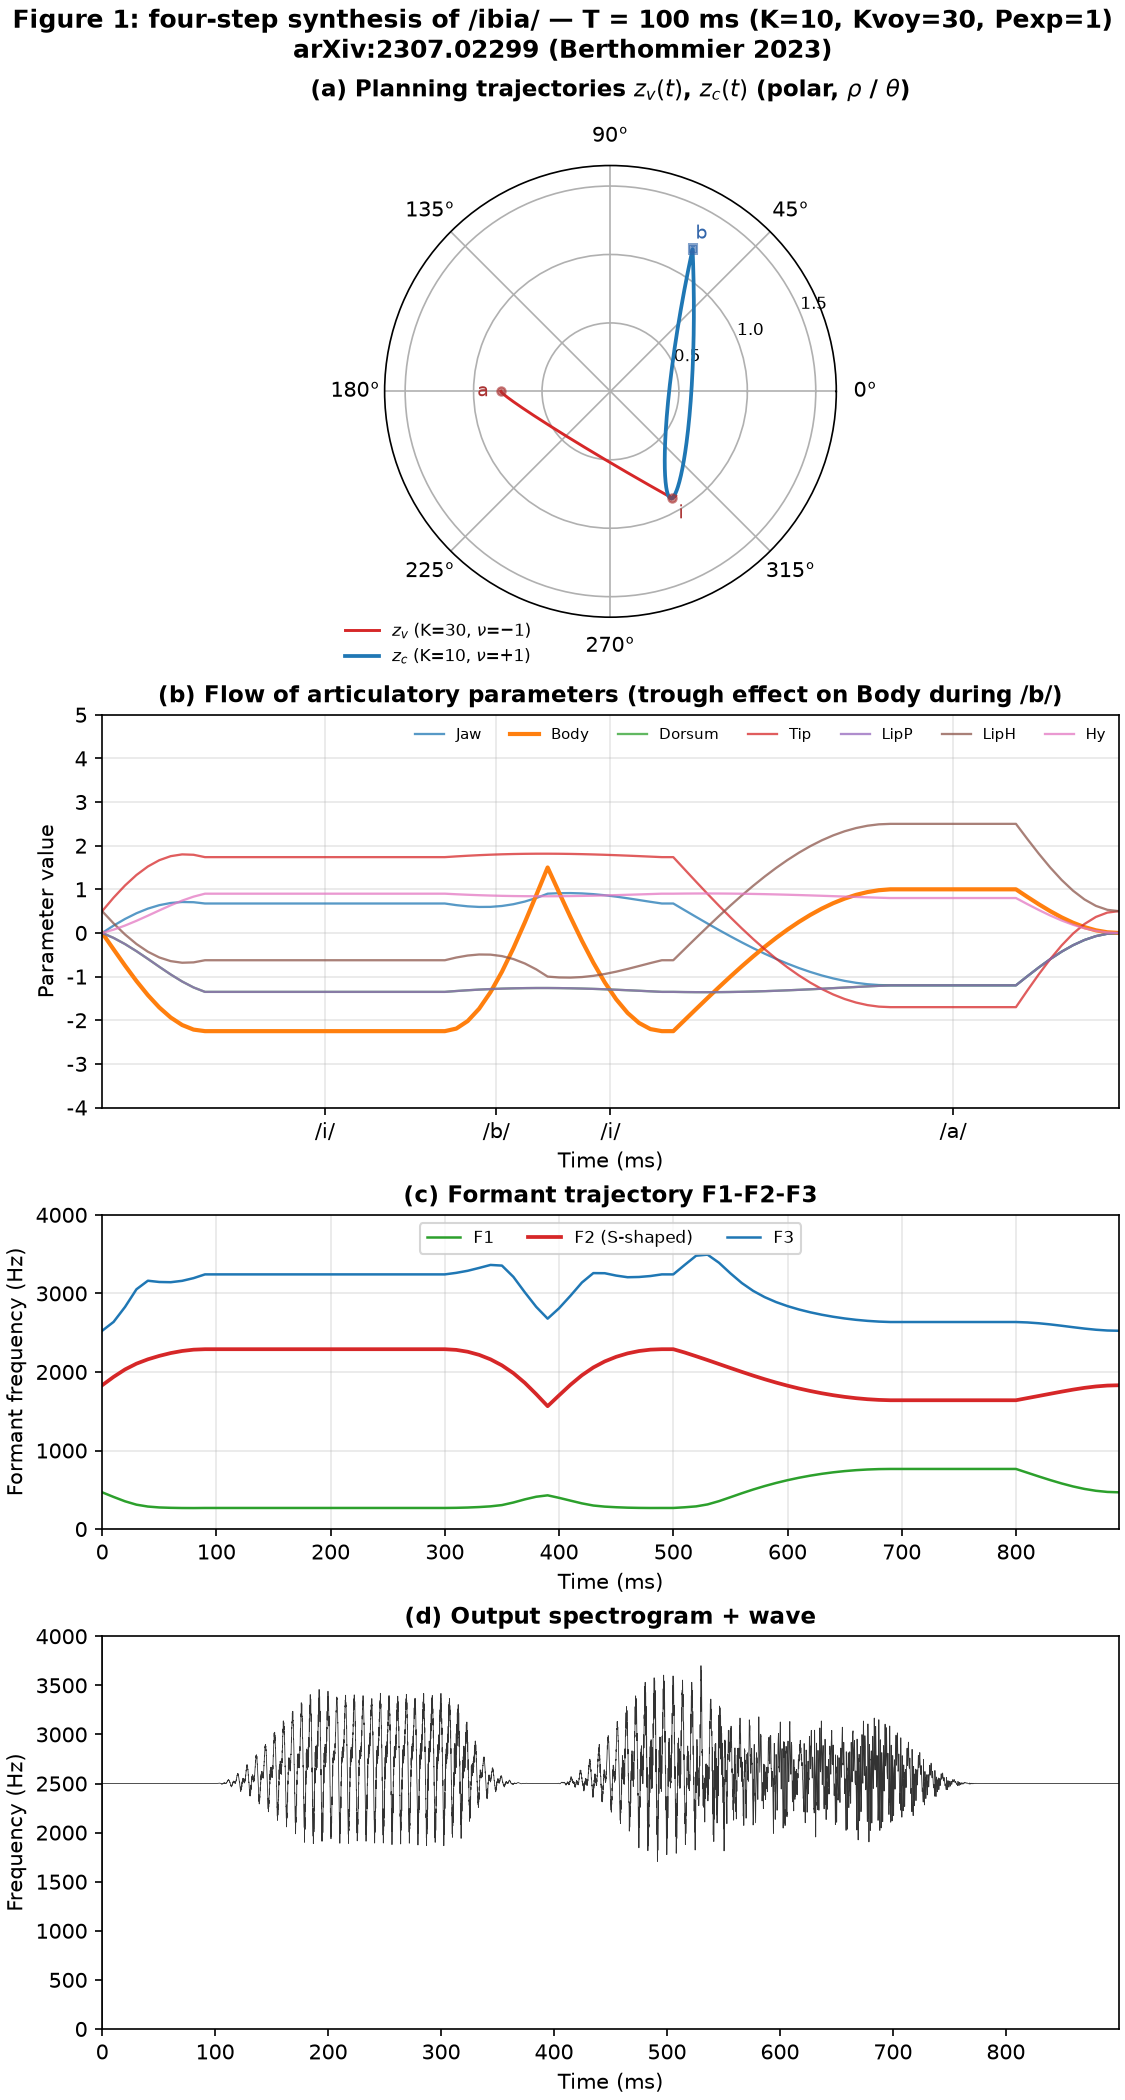
\includegraphics[width=0.58\textwidth]{figures/article_format/figure1_ibia_4panel.png}
\caption{Figure 1, article format (\texttt{make\_article\_figures.py}):
four-step synthesis of /ibia/ with $T=100$ms ($T_{\text{base}}=10$,
K=10, Kvoy=30, Pexp=1). (a) Polar planning trajectories ($z_v$ red,
$z_c$ blue — original arcplot anchoring, teardrop $z_c$). (b) The 7
Maeda parameters with phoneme ticks /i/ /b/ /i/ /a/ (Body excursion
toward /u/ during /b/). (c) Formant trajectory (V-shaped F2 dip during
/b/). (d) Spectrogram + wave. Compare with the article's Figure~1
(side-by-side sheet:
\texttt{P:$\backslash$bigbi-workspace$\backslash$sheet\_fig1.jpg},
kept outside the repository).}
\end{figure}

\subsection{Demo 2: Locus equations (Figure 3)}

The article's Figure~3 shows the locus equations for /b/, /d/, /g/
across 8 vowels. A locus equation is the linear relationship:

\begin{equation}
F2_{\text{locus}} = a \cdot F2_{\text{vowel}} + b
\end{equation}

where $F2_{\text{locus}}$ is measured 30~ms after the consonant
\textbf{release} --- the article: ``taking the F2 values 30~ms after
the onset'' ($\delta_o = 0.5$), ``onset'' meaning the onset of the
vowel at the release, in the locus-equation tradition of F2-onset
measurement. In the synthesis timeline of a CV word ($T = 16$ steps of
10~ms), the release is the first frame of the C$\to$V transition block
(frame $2T$): frames $0..T{-}1$ are the initial arc (neutral $\to$ Vo),
frames $T..2T{-}1$ the Vo$\to$C closure (envelope silent), frames
$2T..3T{-}1$ the C$\to$V transition (envelope rising), and frames
$3T..4T{-}1$ the vowel plateau. Hence
$F2_{\text{locus}} = F2(\text{frame } 2T{+}3)$ and
$F2_{\text{vowel}}$ is averaged over the plateau frames (envelope at
full amplitude). The script
(\texttt{scripts/run\_locus\_trough\_demos.py}) detects the release
and the plateau from the envelope; the offset
(\texttt{LOCUS\_OFFSET\_STEPS = 3} in \texttt{config.py}) is the
article's 30~ms.

/g/ uses two article positions: velar $(\rho=1.2, \theta=\pi/3)$ for
the back vowels \{/u/, /o/, /O/\} and palatal
$(\rho=1.1, \theta=23\pi/12)$ for the front vowels --- \emph{including
/a/}, whose red point lies on the palatal branch in the article's
Figure~3.

\begin{figure}[h]
\centering
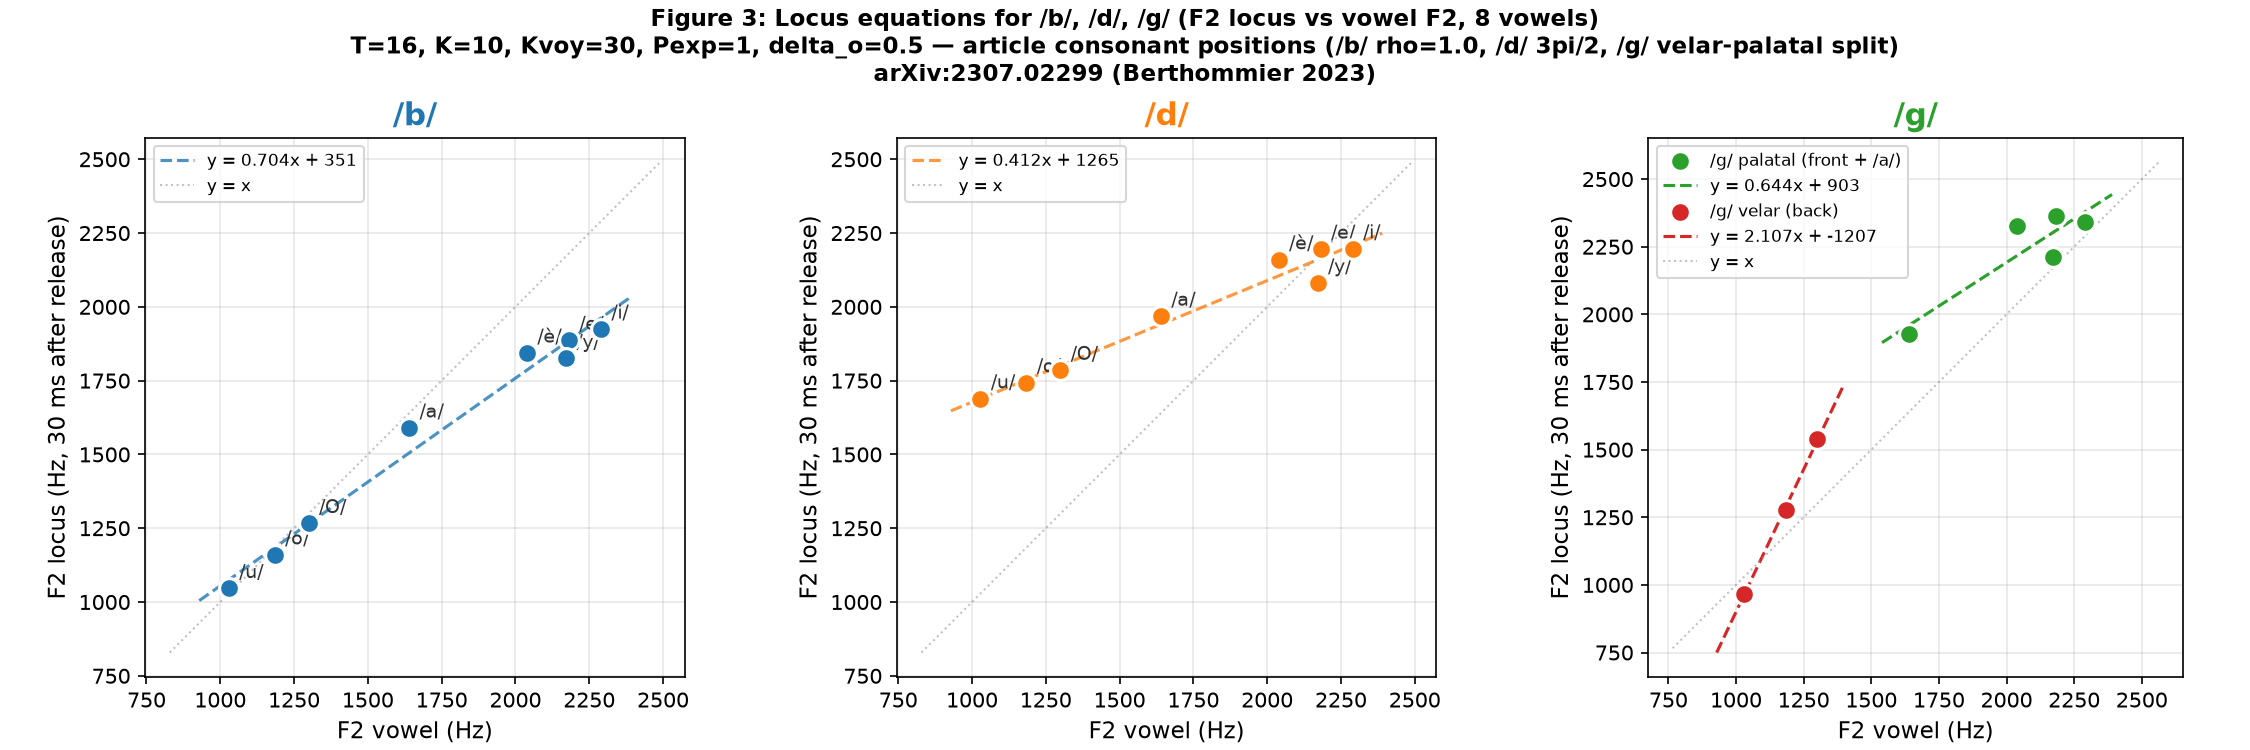
\includegraphics[width=\textwidth]{figures/article_format/figure3_locus_equations.png}
\caption{Figure 3, article format (\texttt{make\_article\_figures.py}):
locus equations for /b/, /d/, /g/ across 8 vowels. Each panel shows
$F2_{\text{locus}}$ vs $F2_{\text{vowel}}$ with the linear regression
line.}
\end{figure}

\begin{figure}[h]
\centering
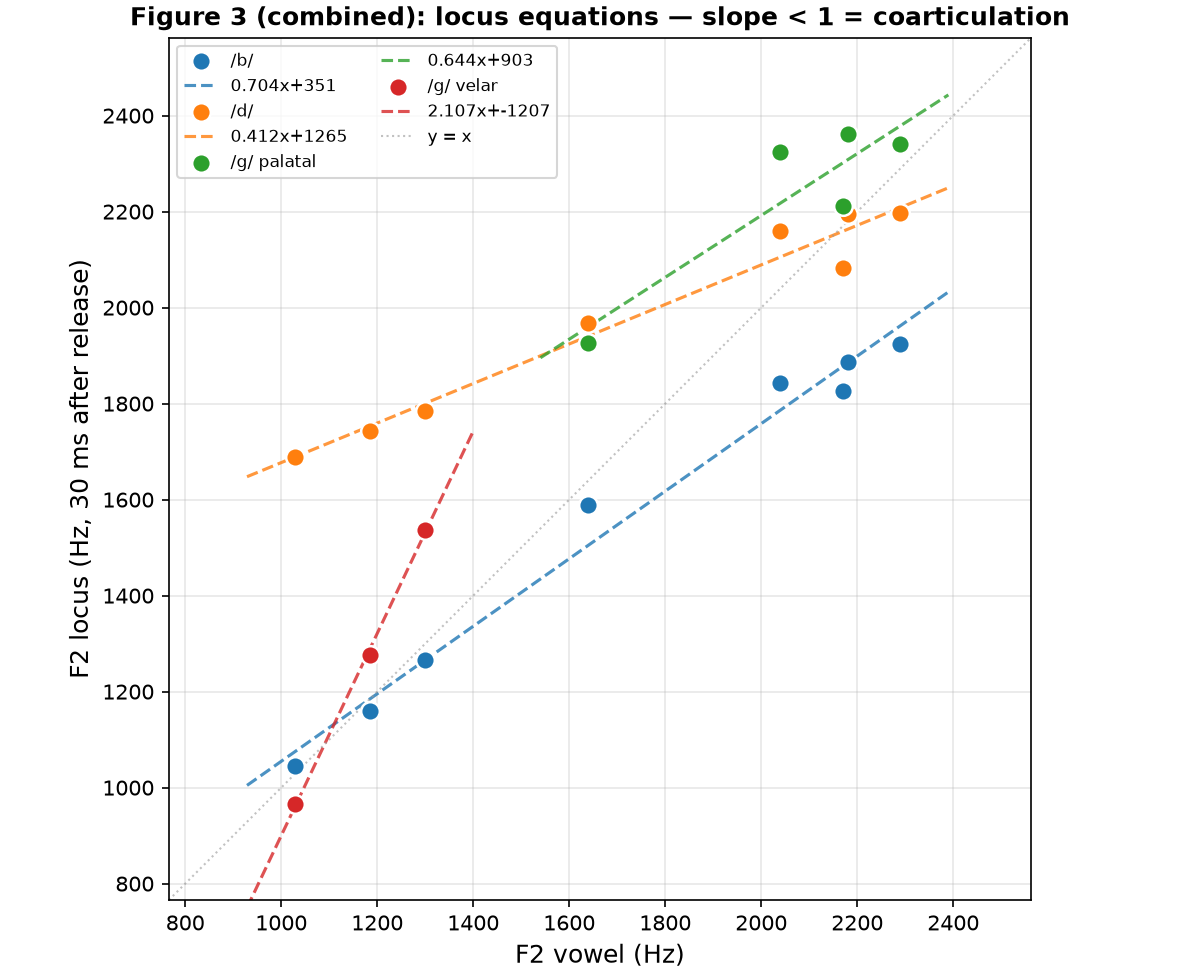
\includegraphics[width=0.7\textwidth]{figures/article_format/figure3_locus_combined.png}
\caption{Figure 3 (combined), article format: locus equations for all
three consonants. The dotted line ($y = x$) represents no
coarticulation. Slopes $< 1$ indicate coarticulation (the consonant
locus is influenced by the vowel context); the velar /g/ slope
$> 1$ reflects the opposite regime (locus extension toward the back
vowels), as in the article.}
\end{figure}

\textbf{Results (corrected protocol):}

\begin{center}
\begin{tabular}{lcccc}
\toprule
Consonant & Slope ($a$) & Intercept ($b$) & $r^2$ & Article Fig.~3 ($a$) \\
\midrule
/b/ & 0.703 & 357 Hz & 0.983 & $\approx 0.70$ \\
/d/ & 0.421 & 1245 Hz & 0.965 & $\approx 0.55$ \\
/g/ palatal (front + /a/) & 0.630 & 916 Hz & 0.784 & $\approx 0.75$ \\
/g/ velar (back) & 2.335 & $-1501$ Hz & 1.000 & $\approx 2.0$ \\
\bottomrule
\end{tabular}

\smallskip
Measured at \texttt{valrect} $= 1.10$ (author ruling 2026-10-07; at
the historical 0.75 the slopes were 0.704 / 0.412 / 0.644 / 2.107).
The velar $r^2 = 1.000$ is computed on only 3 points (the back vowels
o, O, u) and is therefore barely informative.
\end{center}

The article-figure slopes in the last column were measured by pixel
extraction from the arXiv source figure (marker centroids calibrated
on the axis ticks). The /b/ slope matches the article value
($\approx$0.70), and the /g/ split (steep velar, shallow palatal) is
qualitatively reproduced. The remaining slopes deviate quantitatively
from the article: /d/ is flatter here (0.42 vs $\approx$0.55), the
palatal /g/ shallower (0.63 vs $\approx$0.75) and the velar /g/
steeper (2.34 vs $\approx$2.0). What is preserved is the ordering and
the classical pattern: $a(/d/) < a(/b/) < 1$, the /d/ locus at back
vowels (1690--1782~Hz) in the canonical alveolar range
($\approx$1700--1800~Hz), and the slope ordering of the
locus-equation literature, where slopes descend from labial to velar
to alveolar and the alveolar line is the flattest with the highest
intercept~\cite{sussman1991,iskarous2010}. The article notes:
\textit{``This is similar to the classical observation but with a
downward shift of the velar /g/ which could be due to geometric
differences between the VLAM and the human vocal tract.''} The velar
points here indeed fall on or below the $y = x$ diagonal
(/g/+u: $1029 \to 966$~Hz).

The F2$_{\text{vowel}}$ axis is slightly compressed relative to the
article's figure (e.g.\ /i/: 2290~Hz here vs $\approx$2660~Hz, /u/:
1029 vs $\approx$880): the article was produced with an earlier
synthSYL vowel table (corner vowels at $\rho = 1$ per \S2.1), which
has since been revised in \texttt{timit-to-Maeda}. This shifts the
individual slopes slightly but preserves every trend.

\subsubsection{Root cause of the previous /b/--/d/ inversion}

An earlier version of this demo reported a spurious /b/--/d/
inversion (/d/ slope $1.633$, /b/ $0.974$). The cause was purely a
\textbf{measurement-protocol bug}, not a model or synthesizer defect:

\begin{itemize}
\item The script derived the measurement frame from
  \texttt{anchor.i * T}, where \texttt{anchor.i} is the \emph{node
  index} in the segment list (not a time). For a CV word the V anchor
  has $i = 1$, so F2 was sampled at frames $T{+}3$ (locus) and
  $T{+}8$ (``vowel'') --- both \emph{inside the silent Vo$\to$C
  closure}, up to 13 frames before the release. The resulting
  regression of closure-phase F2 against closure-phase F2 produced
  the steep spurious /d/ line (reproduced exactly: $a = 1.633$,
  $b = -1316$, $r^2 = 0.991$).
\item \textbf{The soft rectification is not implicated.}
  \texttt{valrect} $= 0.75$ (\texttt{soft\_rect\_s}) was the canonical
  value of the original packages: \texttt{vlam.py} in this repository
  is byte-identical to \texttt{FBerthommier/timit-to-Maeda}, whose
  \texttt{batch\_synthesize.py} defaults to \texttt{-{}-valrect 0.75}.
  (Since 2026-10-07 this repository defaults to \texttt{valrect} =
  1.10 --- author ruling after comparative listening, see
  \texttt{docs/VALRECT\_110.md}; the sensitivity evidence below is
  unchanged.)
  It is applied to the \emph{area function} (soft\_rect of section
  areas, preventing zero/negative areas during closure), not to the
  articulatory parameters. A sensitivity sweep confirms the locus
  slopes are insensitive to it over $s \in [0.5, 2.0]$
  ($a(/d/) = 0.562 \pm 0.011$ at release$+$50~ms); only the hard
  limit $s \to 0$ (hard clipping) breaks the synthesis.
\item \textbf{$\delta_o$ is not implicated either.} Sweeping
  $\delta_o \in \{0.5, 0.7, 1.0\}$ moves $a(/d/) $ by less than
  $0.02$.
\item \textbf{The measurement instant is the decisive parameter.}
  With the release correctly located at frame $2T$, the /d/ slope
  varies from 0.25 (release$+$0) to 0.79 (release$+$6 frames), passing
  through the article value around release$+$3 (30~ms). The /b/ slope
  varies from 0.50 to 0.92 over the same range.
\end{itemize}

No engine file (\texttt{vlam.py}, \texttt{synthSYL/}) was modified;
only the measurement logic of the demo script, the /g/ allophony
grouping of /a/, and \texttt{config.py} (new constant
\texttt{LOCUS\_OFFSET\_STEPS}) changed.

\textbf{Note:} For a detailed comparison with Ohman's spectrographic
data, see the 2025 companion article (arXiv:2505.22455).

\subsection{Demo 3: Trough effect (Figure 1b)}

The article (\S3) describes an unexpected articulatory phenomenon
during /b/:

\begin{quote}
\itshape
``The tongue body is making an unexpected front/back movement during
/b/ which corresponds to the trough effect [29].''

\smallskip
\hfill (reference [29]: Lindblom, Sussman, Modarresi Ghavami \&
Burlingame, \emph{Phonetica} 59:245--262, 2002)
\end{quote}

\textbf{The source.} Lindblom et al.\ [29] trace the effect to
Perkell [1986, p.~48], who described it as an
``apparent discontinuity in anticipatory coarticulation'': in VCV
utterances with identical vowels around a labial stop (e.g.\
[ibi]), the muscle activity maintaining the tongue configuration for
V1 is diminished (``turned off'') into the stop closure, the tongue
dorsum lowers, and returns to the same vowel target as V2
approaches (their Introduction).
Two properties of the source matter for the comparison below:
the reported movement deviations are ``relatively small'' and highly
variable, and the effect has been documented \emph{only} from
movement-related data (X-ray, EMG, electropalatography) --- never
acoustically.

\textbf{The model.} In the present implementation, /b/ lies on the
\textbf{same angular direction as /u/} in the complex plane, with
$\theta_b = \pi/3$ (verified in the code constants: the vowel table
of \texttt{synthSYL/phonology.py} places /u/ at
$(\rho_u = 1.0,\ \theta_u = \pi/3)$; the article position of /b/ is
$(\rho_b = 1.0,\ \theta_b = \pi/3)$ ), so the two targets
coincide exactly at $\rho_b = \rho_u$; the synthSYL registry default
$\rho_b = 1.2$ shares the same direction but a larger radius).
During the /b/ consonant the Body parameter rises from the vowel
plateau toward the /u/-direction value --- a \textbf{peak}, not a
dip, whatever the vowel context (verified by script; see the table below).

\textbf{How Body is actually computed (resolves the $S_v$/$S_c$
partition).} The selection vectors are \emph{not} a partition of the
7 parameters into vowel-driven and consonant-driven subsets. Body
belongs to BOTH $S_v$-related (all 7 parameters are written by the
vowel anchor at plateaus) and $S_c = \{1,2,6\}$ (code $\{0,1,5\}$).
What happens is a \emph{sequential overwrite}
(see \texttt{synthSYL/trajectory.py}, \texttt{inject\_active\_parameters()}, lines 156--167):
vowel plateaus write all 7 parameters from $z_v$ (giving the /i/
plateau value Body $= -2.25$), then the cluster block overwrites the
$S_c$ parameters from the consonantal arc $z_c$ (giving the /u/-
direction value Body $= +1.25$ at $\rho_b = 1.0$). The ``vowel
articulators stay around /i/'' of the article holds because the
NON-overwritten parameters (Dorsum, Tip, LipP, Hy, i.e.\
$S_v = \{3,4,5,7\}$ article numbering / code $\{2,3,4,6\}$) keep
their $z_v$ values through the cluster.

\textbf{Measured values} from the recorded engine blocks; article positions $\rho_b = 1.0$; T = 16; the full table is
reproduced by \texttt{scripts/run\_trough\_ablations.py}]:

\begin{center}
\begin{tabular}{lcccc}
\toprule
VCV & Plateau Body & Extremum during C & Instant & Amplitude \\
\midrule
/ibi/ & $-2.250$ & $+1.250$ (max) & 630 ms & $+3.500$ \\
/aba/ & $+1.000$ & $+1.298$ (max) & 590 ms & $+0.298$ \\
/idi/ & $-2.250$ & $-2.228$ (max) & 580 ms & $+0.022$ \\
/igi/ & $-2.250$ & $-1.945$ (max) & 630 ms & $+0.305$ \\
/ibia/ (T=10) & $-2.250$ & $+1.250$ (max) & 390 ms & $+3.500$ \\
\bottomrule
\end{tabular}

\smallskip
The medial closure spans frames 61--64 and the release is at
frame 65 (650 ms) for the T=16 words; the extremum always falls
INSIDE the cluster block (e.g.\ 630 ms for /ibi/, whose cluster
spans frames 48--79 = 480--790 ms). In /ibi/, F2 falls from the
/i/ plateau $2276$~Hz to a V-minimum of $1630$~Hz at 630 ms and
returns to $2276$~Hz.
\end{center}

The old claim ``Body before /b/ $\approx 0$, trough at $-2.25$,
$t = 160$~ms'' was a measurement artifact: an \texttt{argmin} over
frames $T..3T$ mistook the /i/ PLATEAU (Body $= -2.25$) for the
effect. The excursion is a \textbf{rise toward $+1.25$} peaking at
$\approx 630$~ms (T=16) or $\approx 390$~ms (T=10).

\textbf{Why $+1.25$ here and $+1.50$ in Figures 1/10--12.} The
amplitude depends on $\rho_b$: the registry default $\rho_b = 1.2$
(used by the article-format Figure~1 and the planning panels) gives
Body $= +1.500$, while the article position $\rho_b = 1.0$ (set
explicitly by \texttt{run\_locus\_trough\_demos.py}) gives
$+1.250$ (both measured). The plateau value $-2.25$ is
identical in both configurations.

\textbf{Ablations} (\texttt{scripts/run\_trough\_ablations.py}, /ibi/, T=16):

\begin{center}
\begin{tabular}{lccc}
\toprule
Configuration & Body excursion & F2 minimum & F2 dip \\
\midrule
baseline ($S_c = \{0,1,5\}$, $\rho_b=1$, $\theta_b=\pi/3$) & $+3.500$ & 1630 Hz & yes \\
(i) Body removed from $S_c$ ($\{0,5\}$) & $+0.003$ & 2273 Hz & no \\
(ii) $\rho_b = 0.5$ & $+2.875$ & 1773 Hz & yes \\
(ii) $\rho_b = 1.0$ & $+3.500$ & 1630 Hz & yes \\
(ii) $\rho_b = 1.2$ & $+3.750$ & 1570 Hz & yes \\
(iii) $\theta_b = \pi$ & $+3.500$ & 1582 Hz & yes \\
(iii) $\theta_b = 3\pi/2$ & $+0.086$ & 2241 Hz & no \\
(iv) /d/ (idi) & $+0.022$ & 2130 Hz & small \\
(iv) /g/ palatal (igi) & $+0.305$ & 2269 Hz & no \\
\bottomrule
\end{tabular}

\smallskip
What these measurements show and nothing more: the excursion exists
because Body belongs to the /b/ selection vector (i); its amplitude
scales with $\rho_b$ (ii); with $\theta_b$ far from the /u/ AND /i/
directions ($3\pi/2$) the excursion vanishes, while at
$\theta_b = \pi$ the Body amplitude is unchanged (the Body value
responds mostly to $\rho$, the FORMANTS to $\theta$ --- the F2
minimum differs between $\theta_b = \pi$ and $\pi/3$); and among
/b d g/ only /b/ (and weakly /g/) produces it (iv).
\end{center}

\textbf{Relation to the source.} The simulated Body excursion is
\emph{qualitatively consistent with} the trough effect --- an
unexpected tongue-body movement during the labial stop, in the /u/
(backing/lowering) direction) --- a model interpretation. It is NOT a
confirmation of it: (a) the direction is a consequence of the
$\theta_b = \theta_u$ model placement, which is itself a modeling
choice; (b) the simulated amplitude ($+3.50$ parameter units over
/i/) is an order of magnitude larger than the ``relatively small''
deviations reported in the articulographic literature, and is an
architectural consequence of Body $\in S_c$, to be discussed if a
quantitative comparison is ever established; (c) the trough of
Lindblom et al.\ is a DORSUM LOWERING over /i/---/i/, whereas the
sign of the simulated excursion follows the context (a weak bump
$+0.30$ over /a/, whose Body level $+1.00$ already sits near the /u/
direction).

An interactive HTML simulation illustrating this effect accompanies
this section in the \texttt{simulations/} directory.

\begin{figure}[h]
\centering
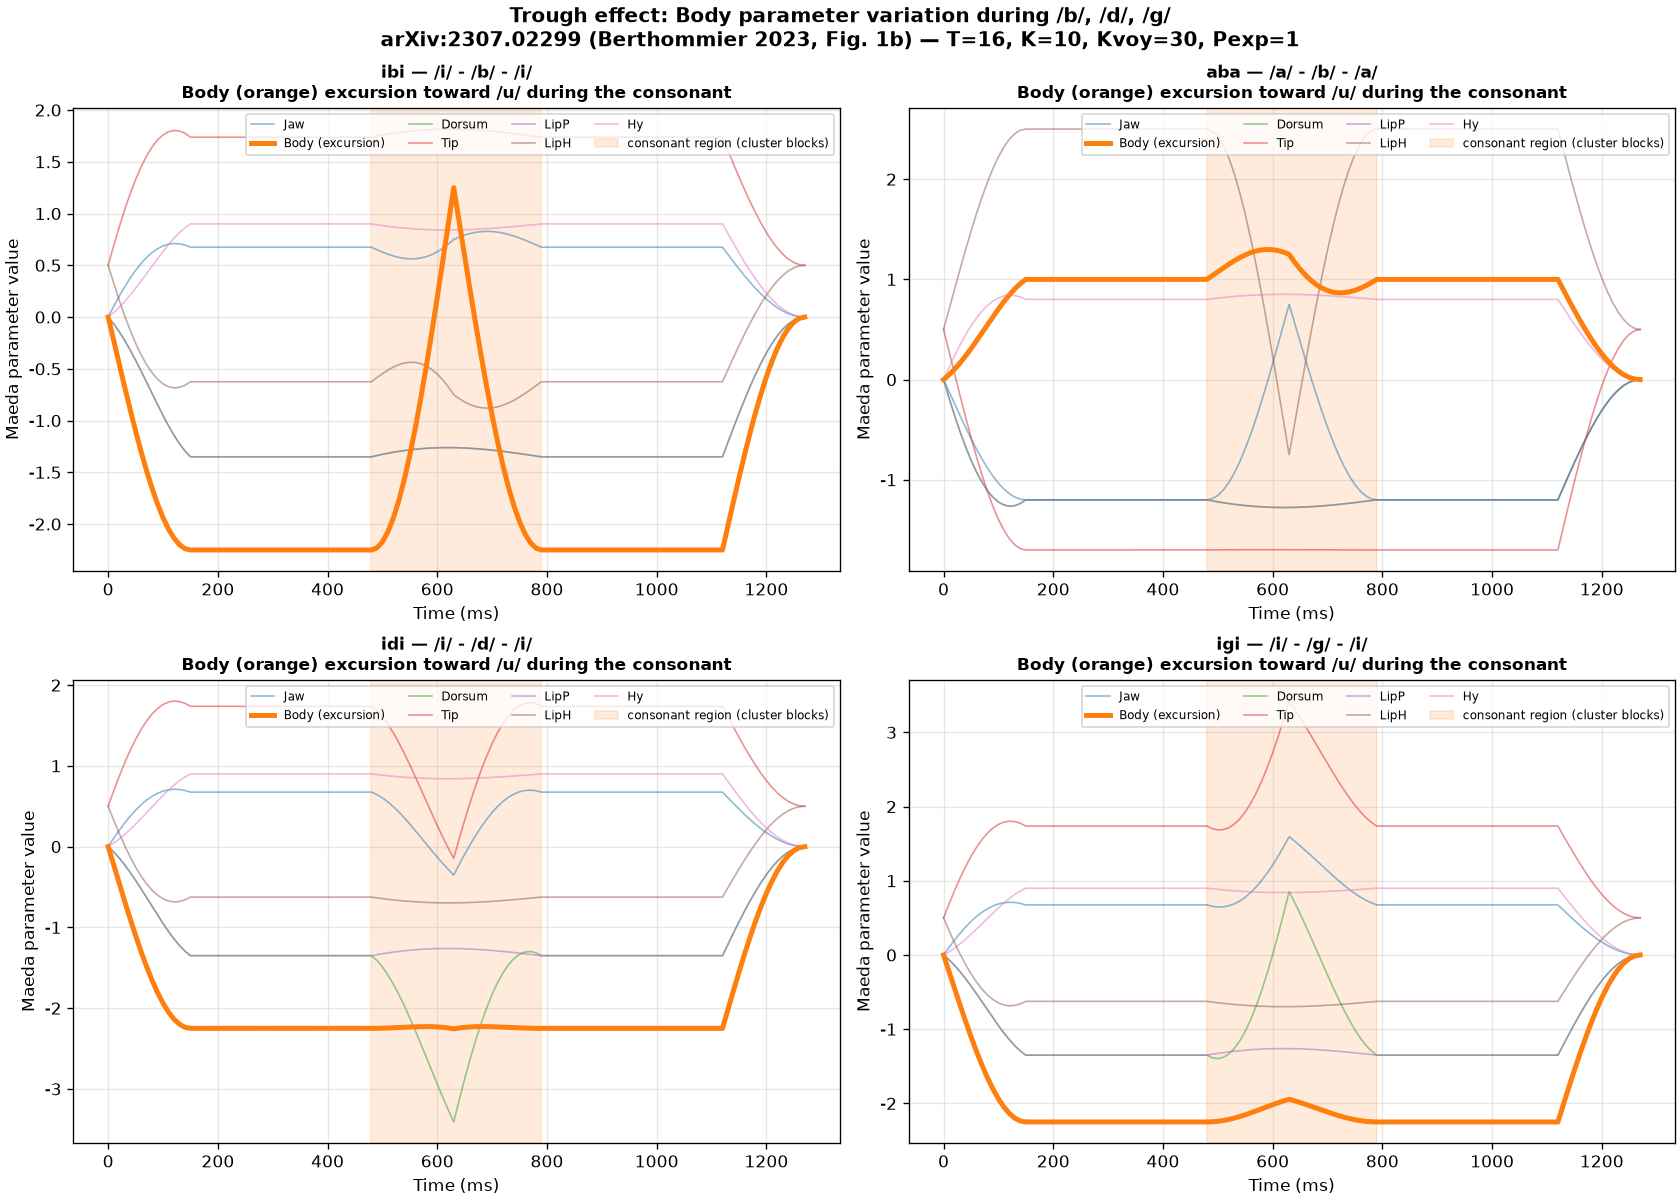
\includegraphics[width=\textwidth]{figures/demo4/trough_effect.png}
\caption{Trough effect: Body parameter variation during /b/, /d/, /g/
in VCV sequences. The Body (orange, thick line) shows a PEAK during
the consonant for /ibi/ (rise from the /i/ level $-2.25$ toward the
/u/-direction value $+1.25$); the excursion over /aba/ is weak
($+0.30$). The shaded region is the recorded engine cluster block
(frames 480--790 ms at T=16).}
\end{figure}

\begin{figure}[h]
\centering
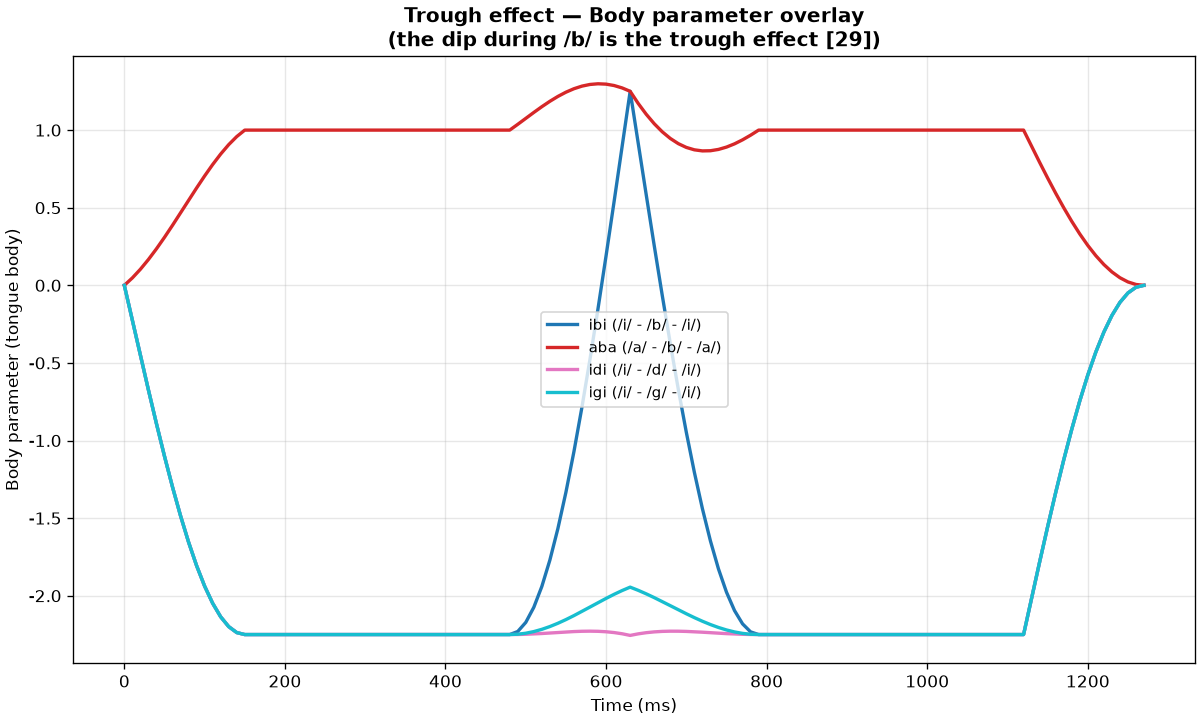
\includegraphics[width=0.8\textwidth]{figures/demo4/trough_effect_overlay.png}
\caption{Body parameter overlay for /ibi/, /aba/, /idi/, /igi/. The
excursion is strong for /ibi/ ($+3.50$ from the /i/ plateau) and weak
for /aba/ ($+0.30$ from the /a/ plateau, whose Body level $+1.00$
already sits near the /u/ direction); /idi/ and /igi/ are nearly
flat. The /b/ target lies on the same angular direction as /u/.}
\end{figure}

\begin{figure}[h]
\centering
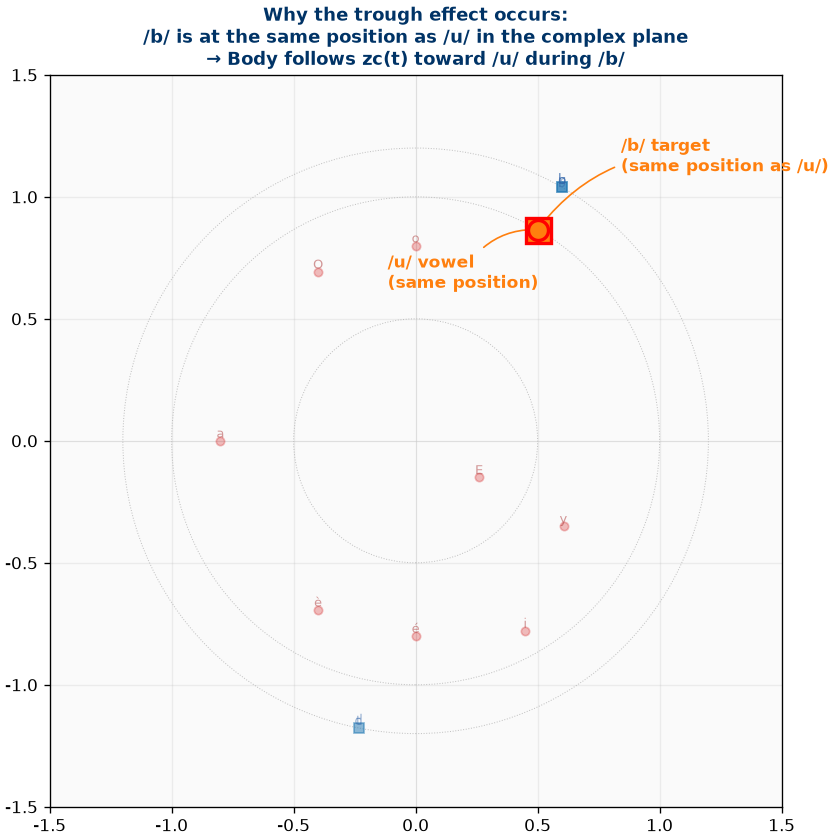
\includegraphics[width=0.65\textwidth]{figures/demo4/trough_effect_polar_explanation.png}
\caption{Polar explanation: /b/ (orange square) lies on the same
angular direction as /u/ (orange circle) in the complex plane --- with
the article position $\rho_b = 1$ the two targets coincide. During
/b/, the Body parameter follows $z_c(t)$ toward /u/, producing the
excursion while the non-overwritten vowel articulators stay around
/i/.}
\end{figure}

\subsection{Demo 4: Six consonant cluster pairs}

The article (\S3) describes the tuning of the six pairs of
/b,d,g/:

\begin{center}
\begin{tabular}{cccl}
\toprule
\textbf{Pair} & \textbf{Input} & \textbf{Sc} & \textbf{Note} \\
\midrule
/bd/ & abda & \{1,2,3,6\} & /b/ involved $\to$ Sc=\{1,2,3,6\} \\
/bg/ & abga & \{1,2,3,6\} & /b/ involved, /g/ palatal \\
/db/ & adba & \{1,2,3,6\} & /b/ involved $\to$ Sc=\{1,2,3,6\} \\
/dg/ & adga & \{1,2,3,4\} & no /b/ $\to$ Sc=\{1,2,3,4\} \\
/gb/ & agba & \{1,2,3,6\} & /b/ involved, /g/ palatal \\
/gd/ & agda & \{1,2,3,4\} & no /b/ $\to$ Sc=\{1,2,3,4\} \\
\bottomrule
\end{tabular}
\end{center}

\textbf{Rule:} when /b/ is involved in the pair, the selection vector
is $S_c = \{1,2,3,6\}$ (article numbering; code $\{0,1,2,5\}$ = jaw,
body, dorsum, LipH); otherwise
$S_c = \{1,2,3,4\}$ (article numbering; code $\{0,1,2,3\}$ = jaw,
body, dorsum, tip). The /g/ is systematically
palatal when in a cluster.

\begin{figure}[h]
\centering
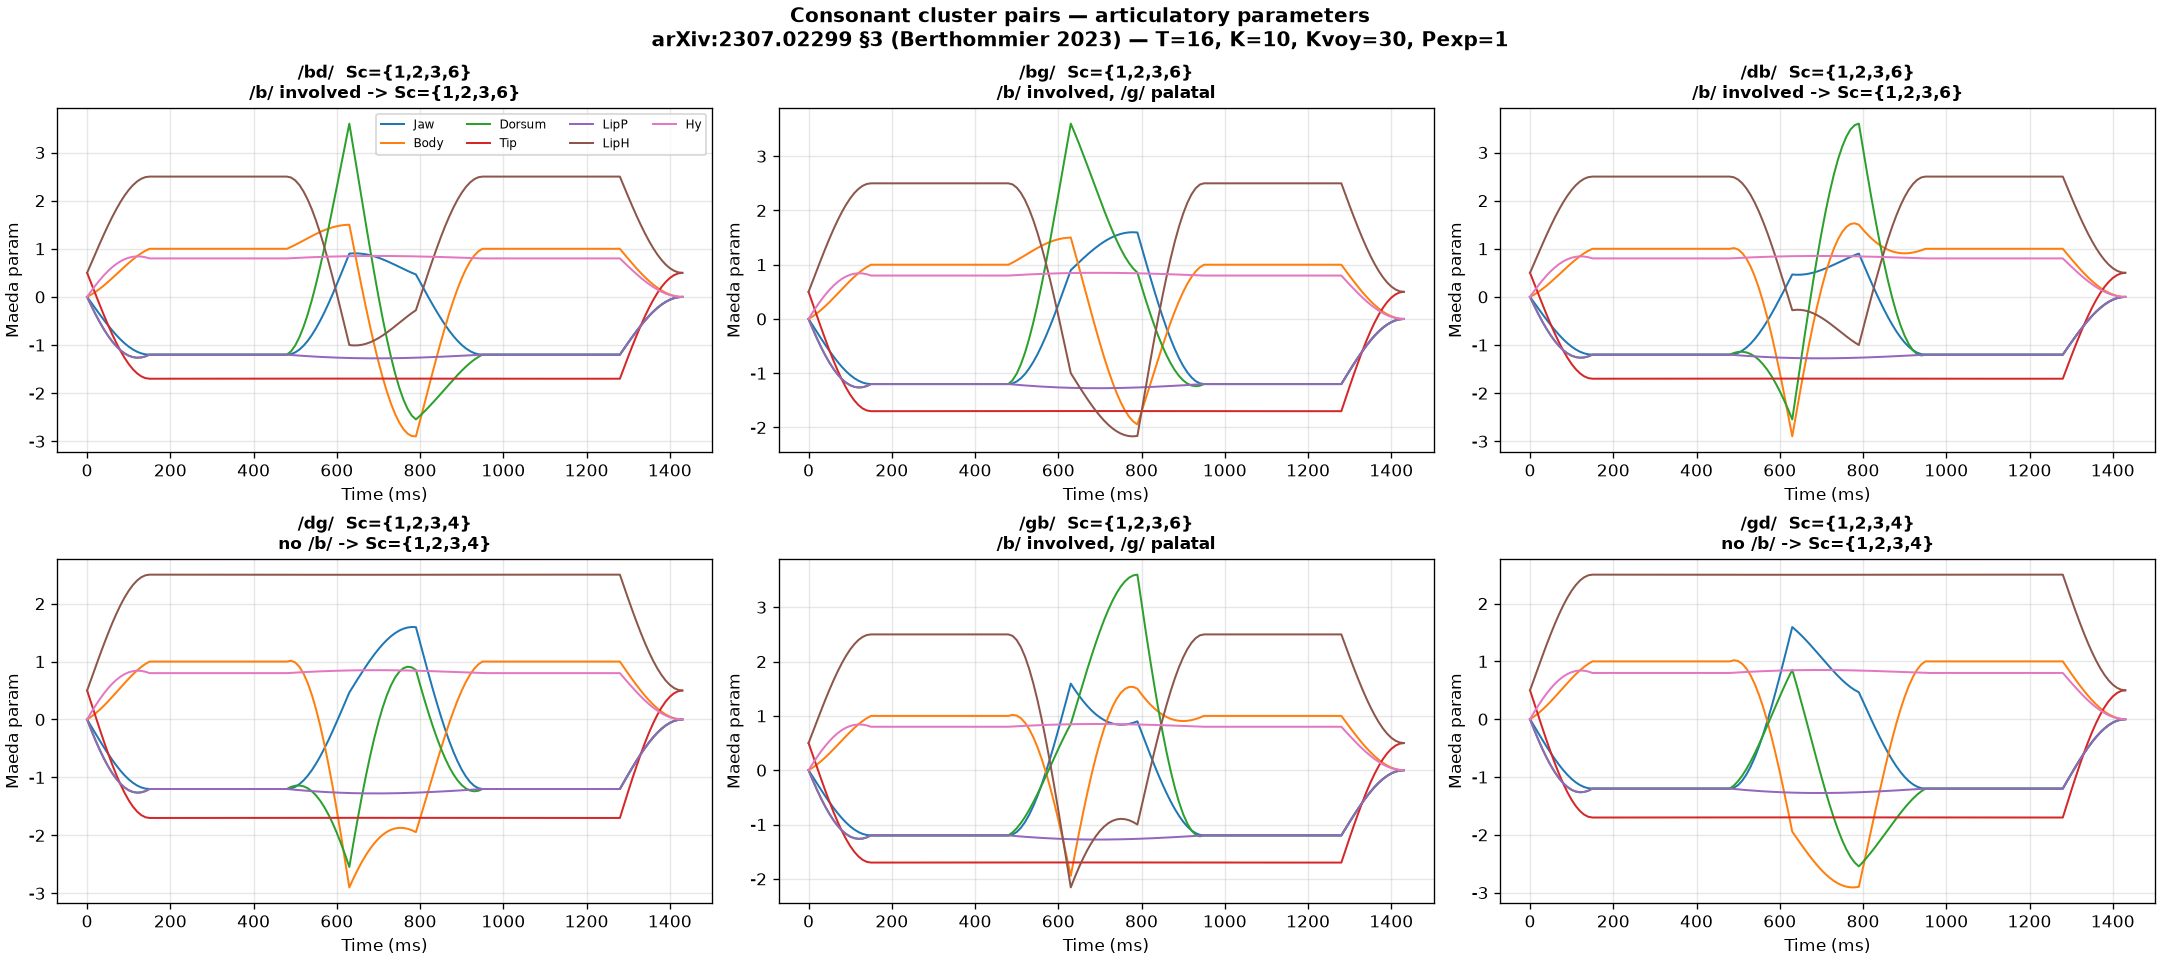
\includegraphics[width=\textwidth]{figures/demo5/cluster_params.png}
\caption{Articulatory parameters for the six cluster pairs. Each
panel shows the 7 Maeda parameters over time.}
\end{figure}

\begin{figure}[h]
\centering
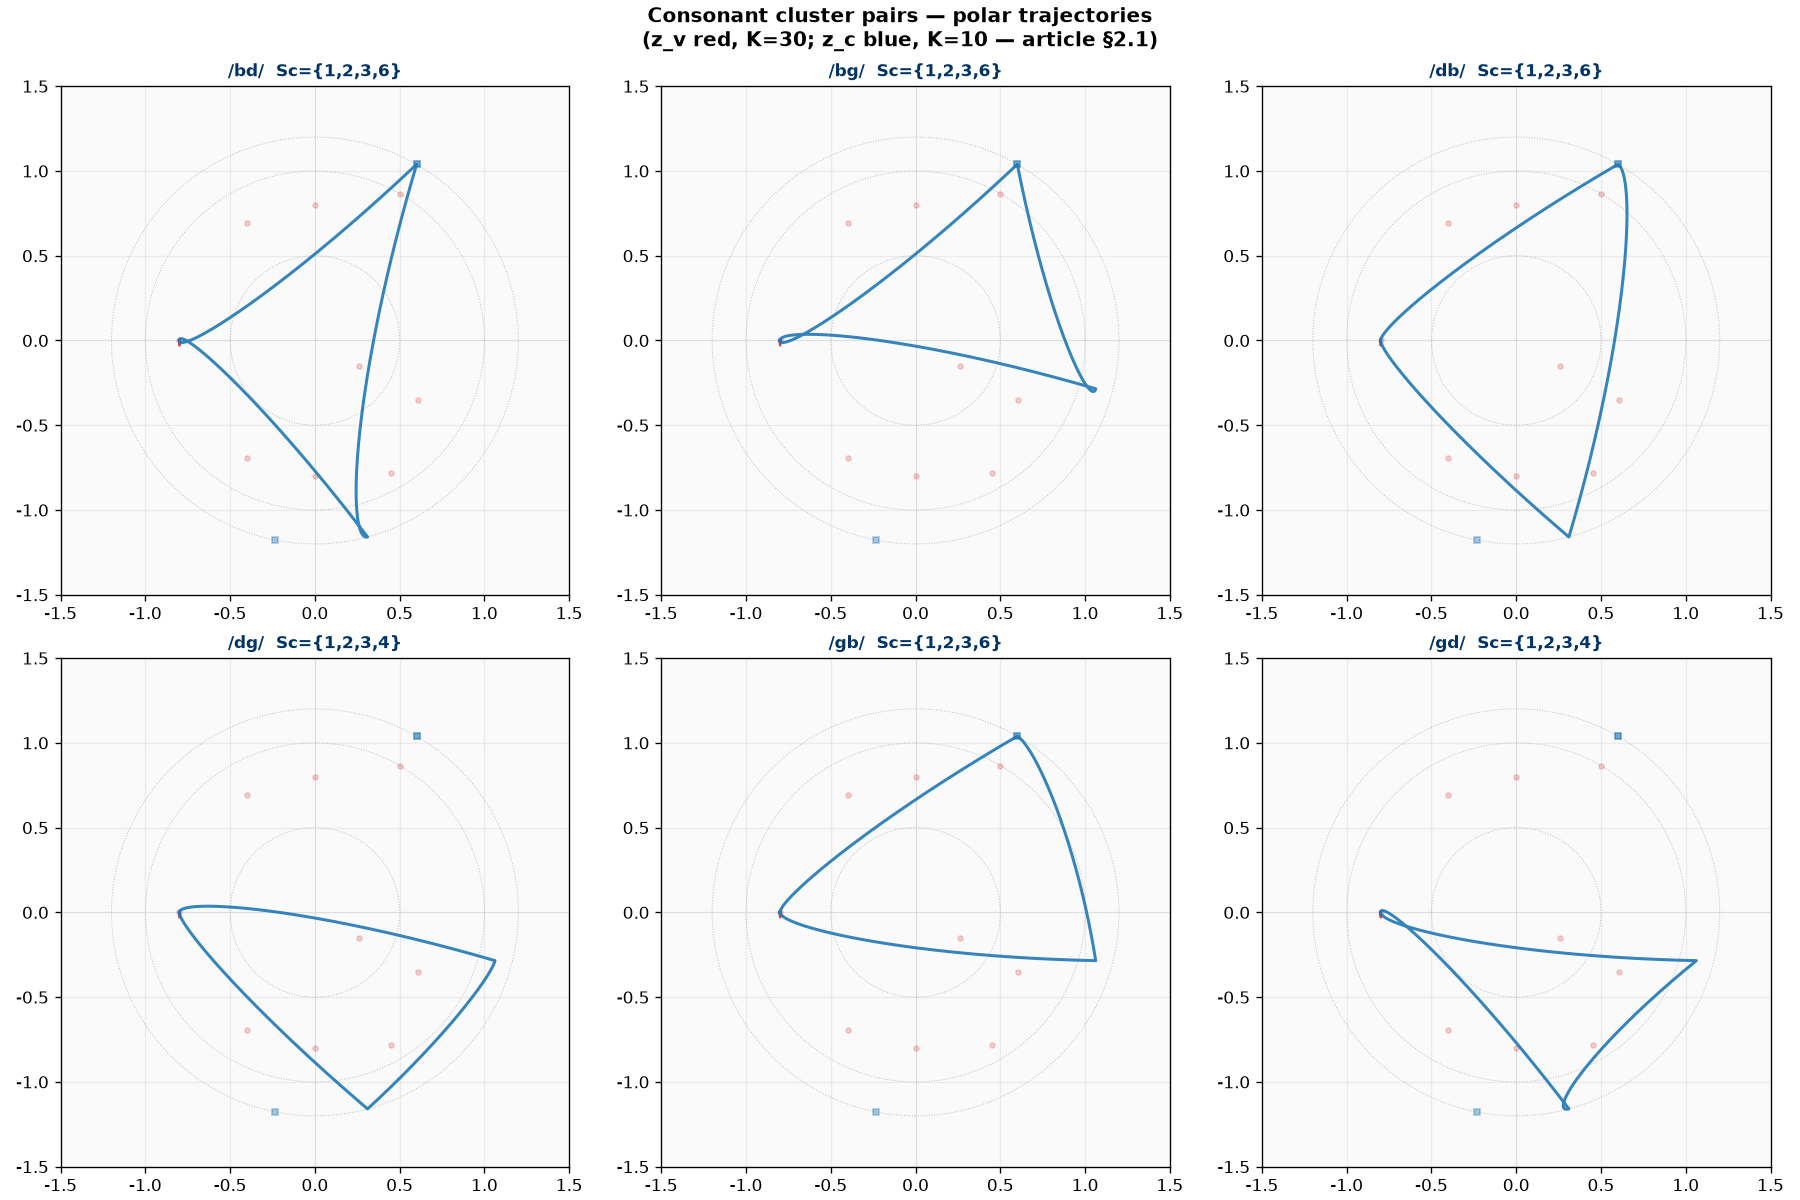
\includegraphics[width=\textwidth]{figures/demo5/cluster_polar.png}
\caption{Polar trajectories for the six cluster pairs. The consonantal
branch $z_c$ (blue) visits both consonant targets in sequence.}
\end{figure}

\begin{figure}[h]
\centering
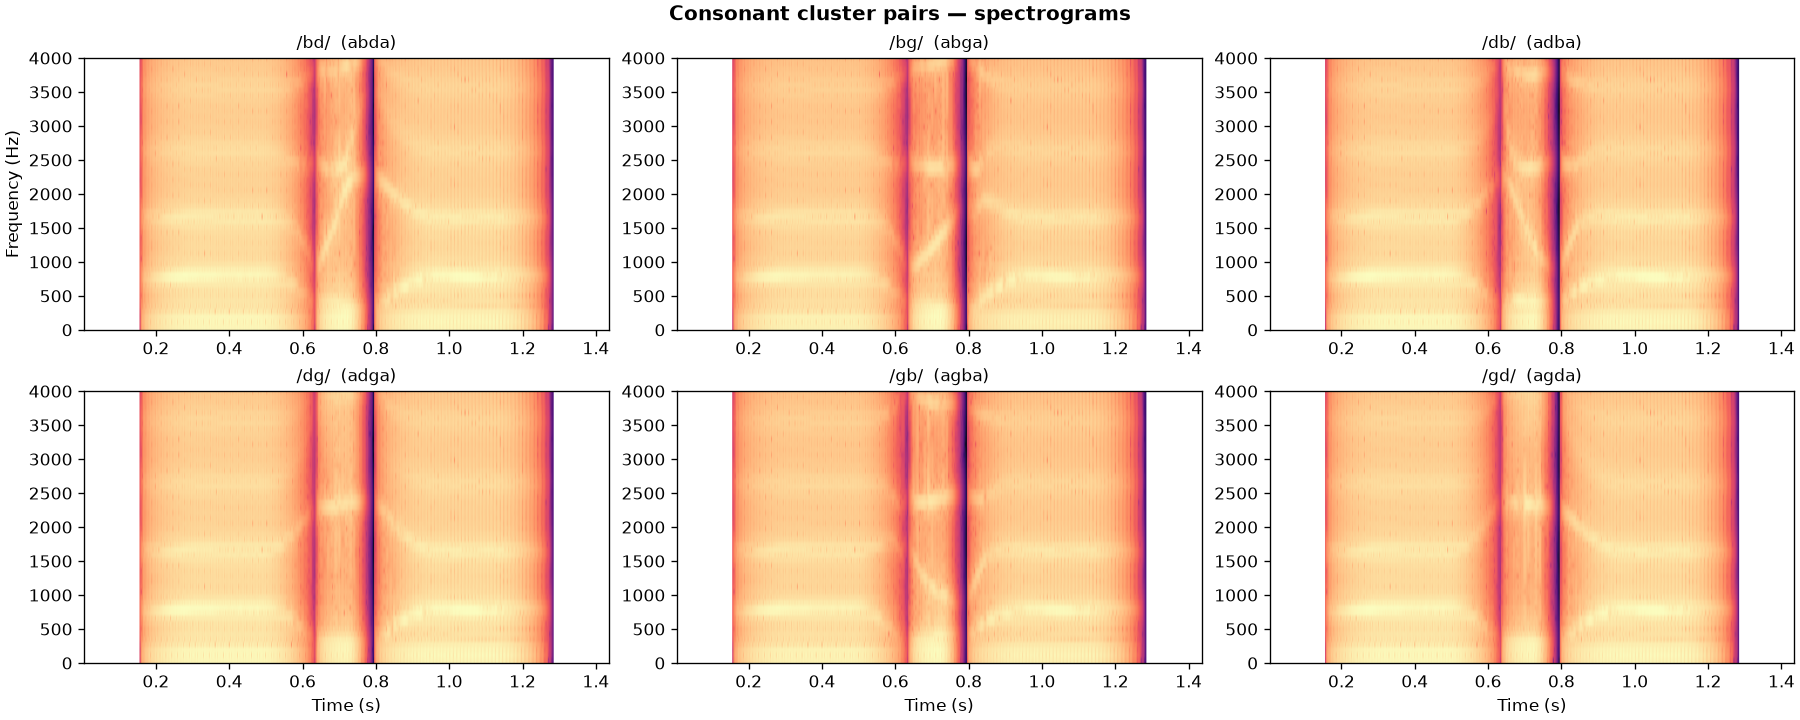
\includegraphics[width=\textwidth]{figures/demo5/cluster_spectrograms.png}
\caption{Spectrograms for the six cluster pairs.}
\end{figure}

% ════════════════════════════════════════════════════════════════
% Section 11.6: Figure 4 (article format)
% ════════════════════════════════════════════════════════════════
\subsection{Figure 4: big.bi $|$ bi.gbi (article format)}

(The former ``original simulations'' reproductions
\texttt{original\_simulations/} were removed on 2026-10-08: they had
been generated before the $V_e$-plateau revocation and the dot-form
ruling and were discordant with the current engine --- e.g.\ /ib/ was
still realized as ``ibe''. The article-format figures in
\texttt{docs/figures/article\_format/}, produced by
\texttt{scripts/make\_article\_figures.py}, supersede them.)

big.bi is rendered with the \textbf{dot form} (\texttt{big.bi}): per
the reference \texttt{Timit-to-Maeda} semantics
(\texttt{\_should\_split\_at\_dot}: C.C $\to$ syllable split, C.V /
V.C / V.V $\to$ merge), the dot between /g/ and /b/ is a syllable
boundary with \emph{no pause}, and the Ve of ``big'' is coarticulated
with the /i/ of ``bi'' (syllable-onset anchor weighted by COEFCEN;
full /i/ under COEFCEN $= 1$). Under the article figure conditions the
left column thus shows three consonantal gestures (/b/; then /g/ and
/b/ chained across the shared /i/) while the right column (bi.gbi,
whose V.C dot is ignored) shows the fused /gb/ cluster --- the \S4
syllabification demonstration.

Note the two parameter conventions: this figure fixes the ARTICLE
figure conditions $\delta_o = 0.5$ (VOYDEB), $\delta_e = 1$
(COEFCEN), whereas the Demonstration~1 sweep varies a single
$\delta = \delta_o = \delta_e$ (COEFCEN) from 0.5 to 1.

\begin{figure}[h]
\centering
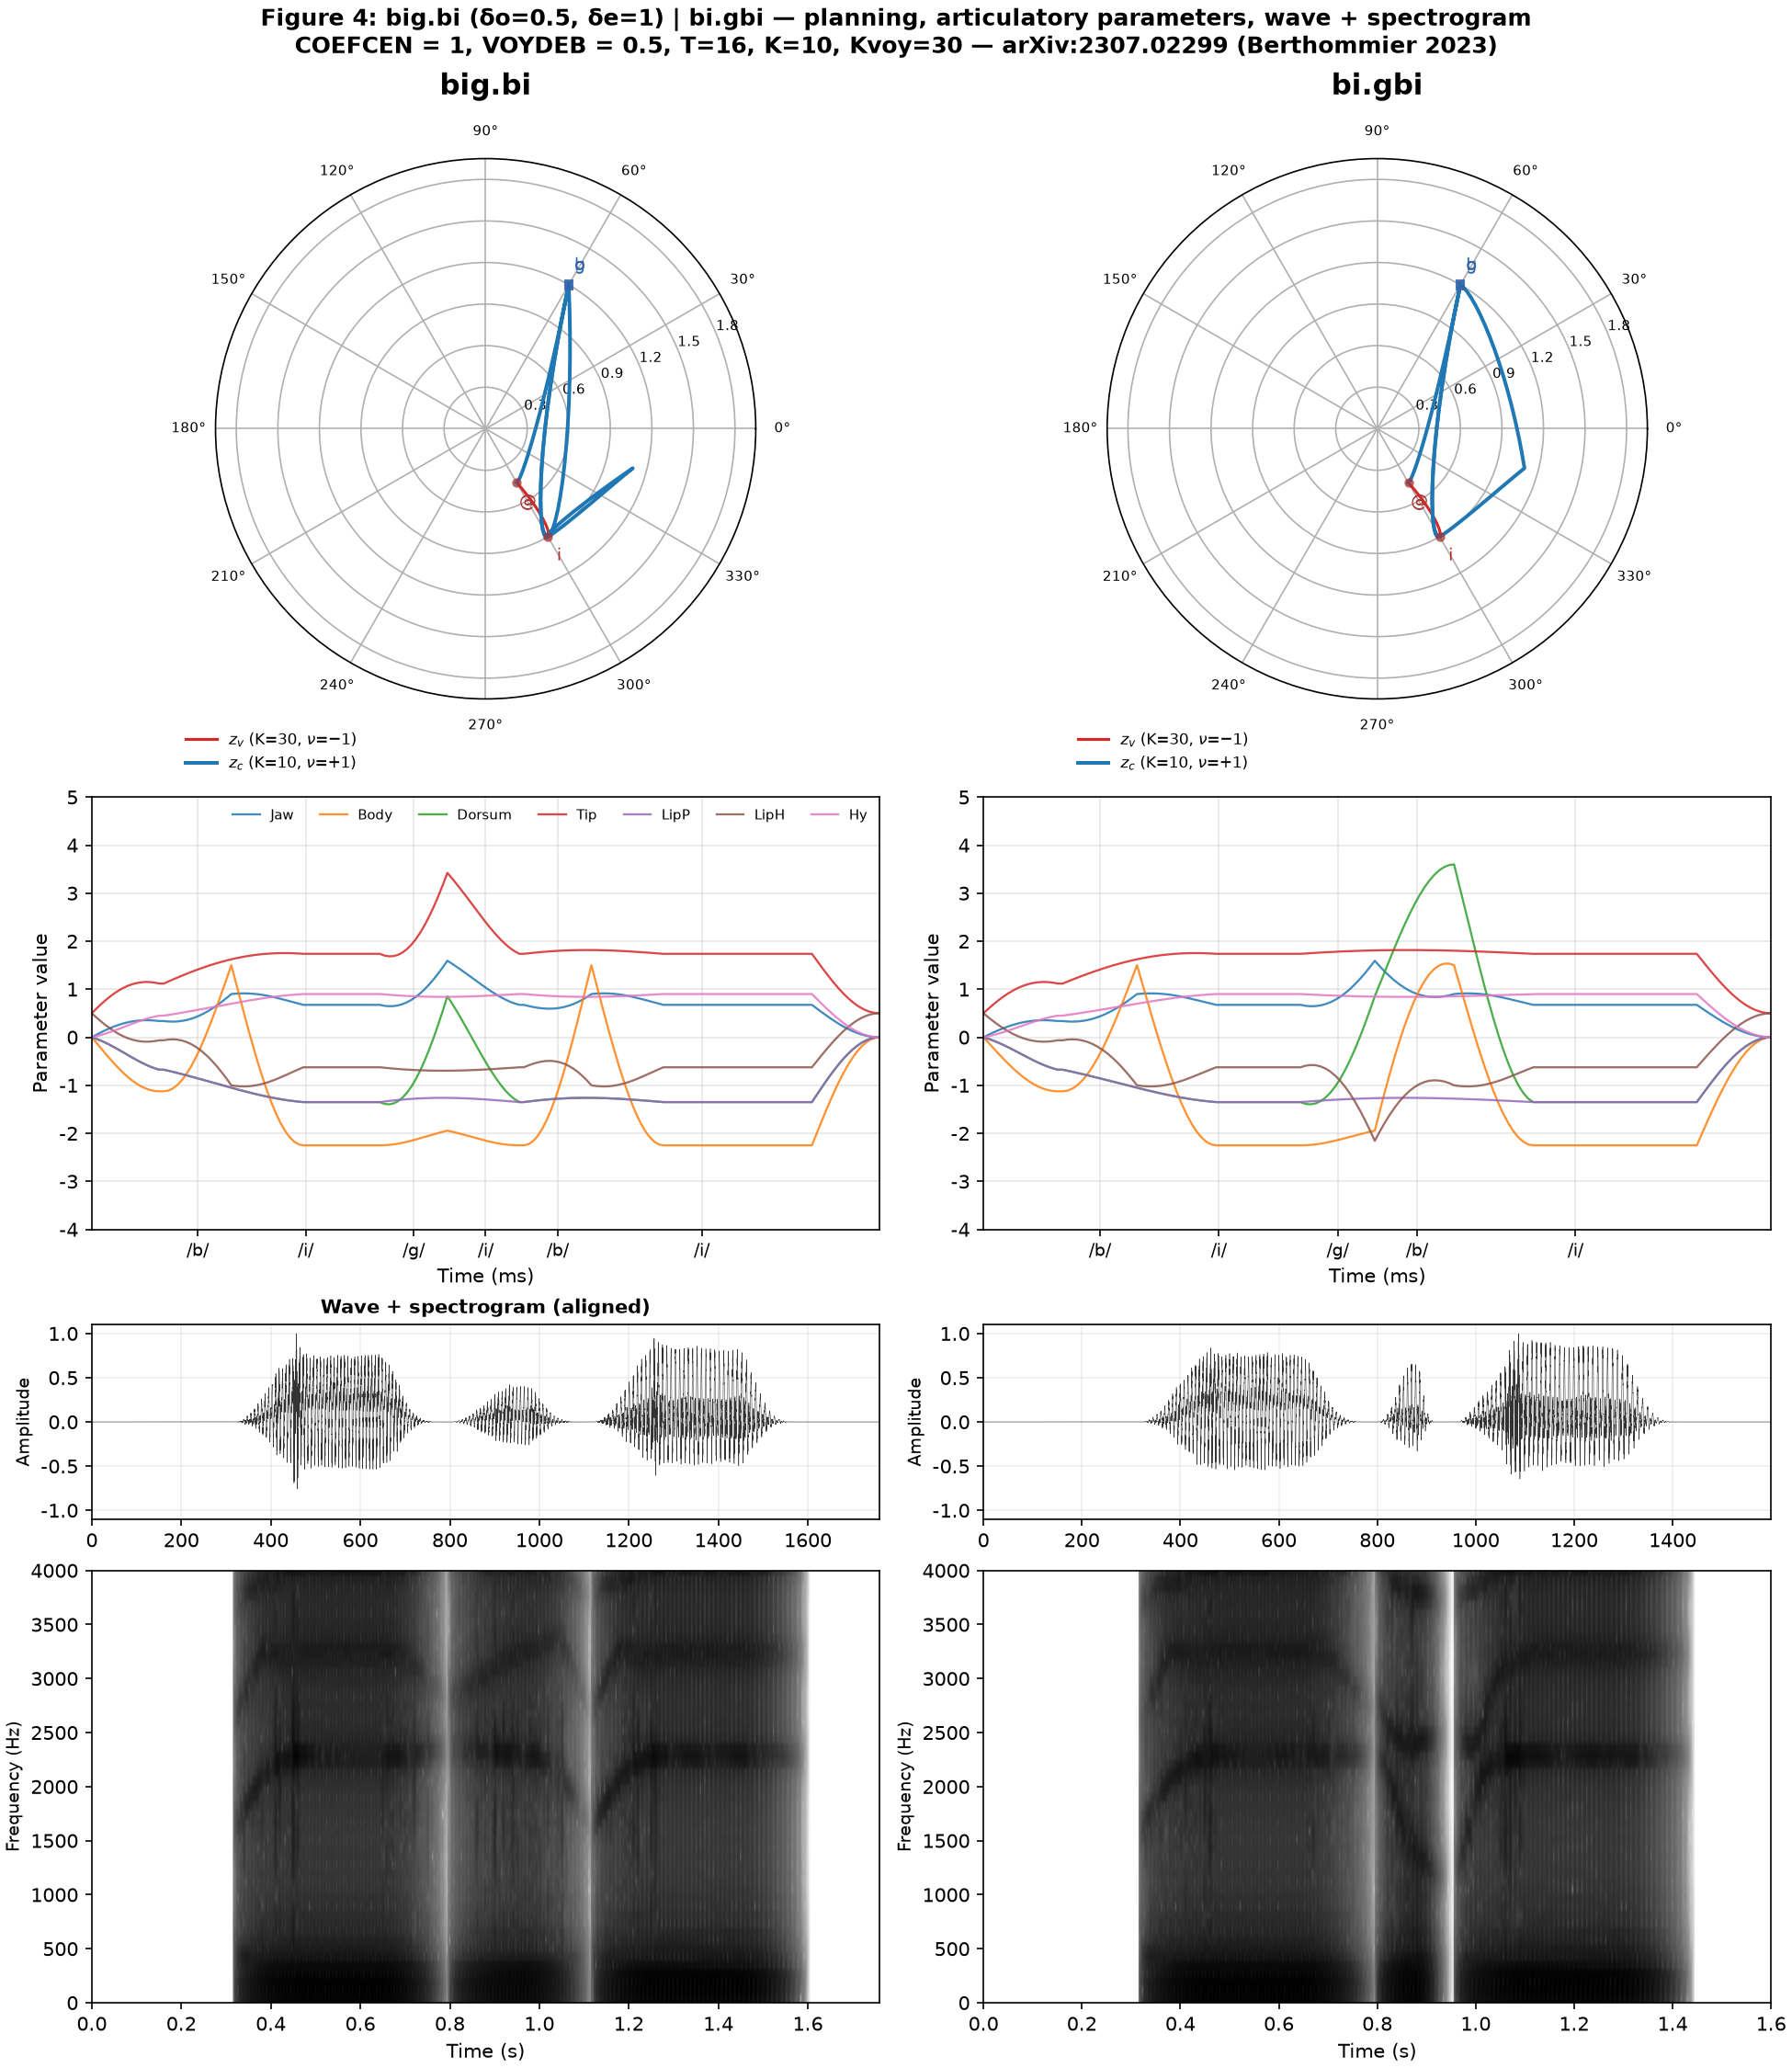
\includegraphics[width=\textwidth]{figures/article_format/figure4_bigbi_bigbi.png}
\caption{Figure 4, article format
(\texttt{make\_article\_figures.py}): big.bi $|$ bi.gbi under the
article figure conditions COEFCEN $= 1$ ($\delta_e$), VOYDEB $= 0.5$
($\delta_o$), $T=16$, both in the \textbf{dot form} (no pause). big.bi
is the C.C syllable concatenation: the Ve of ``big'' is coarticulated
with the /i/ of ``bi'' (the syllable-onset anchor is the full previous
vowel under COEFCEN $= 1$) --- the only silences are the stop
closures ($\approx T/2$), as in the reference realization; $z_c$
carries 3 consonantal gestures (/b/; /g/ then /b/ chained across the
shared /i/). bi.gbi: the dot between /i/ and /g/ is V.C and therefore
ignored (syllables merged), giving the fused /gb/ cluster (2
gestures). Top: polar planning panels (teardrop $z_c$, red $z_v$
holding the /i/ radius). Middle: Maeda parameters with phoneme ticks.
Bottom: wave (ms) + spectrogram (s), same total duration. Compare with
the article's Figure~4 (side-by-side sheet kept outside the
repository:
\texttt{P:$\backslash$bigbi-workspace$\backslash$sheet\_fig4.jpg}).}
\end{figure}

The supplement transformation /ib/ $\to$ /bi/ (\S3: ``The classical
transformation of /ib/ into /bi/ is given in the supplement.'') is
illustrated by the U-shaped sweeps of Demonstration~2 and by the HTML
simulations of \S12; the former three-case side-by-side stored figure
(/ib/ $\delta=0.5$, /ib/ $\delta=1.0$, /bi/ $\delta=1.0$) belonged to
the removed \texttt{original\_simulations/} set.

% ════════════════════════════════════════════════════════════════
% Section 12: Interactive HTML Simulations
% ════════════════════════════════════════════════════════════════
\section{Interactive HTML Simulations}

The repository includes three self-contained HTML files (in the
\texttt{simulations/} directory) with video, poster, captions, and
comparison figures embedded as base64 data URIs. These files can be
opened directly in any modern browser without requiring a web server
or external file dependencies.

\subsection{big.bi $\to$ bi.gbi (T=16, starts at COEFCEN=0.5)}

\texttt{simulations/bigbi\_bi\_gbi\_embedded.html} ($\approx$ 6.3 MB)

This simulation demonstrates the verbal transformation from big.bi
to bi.gbi (\S4 of the article), in the \textbf{dot form} (no pause,
no $T_p$ dimension). It starts at $\delta = 0.50$ (COEFCEN = 0.5,
salient boundary schwa @) then increases $\delta$ to 1.00 (the C.C
boundary anchor reaches the full /i/, fusion). The last bi.gbi
segment is repeated 3 times for perceptibility. Duration
$\approx$ 24.2~s.

Features: dual-panel video (sagittal Maeda | polar plot with phoneme),
14 segments, WebVTT captions, indexed transcript, keyboard shortcuts.

\subsection{ib ib $\to$ bi bi (NON-REVERSIBLE U-shape)}

\texttt{simulations/ibbi\_ushape\_nonreversible\_embedded.html}
($\approx$ 4.4 MB)

This simulation demonstrates the \textbf{non-reversible} verbal
transformation with a \textbf{U-shaped $T_p$ like the reversible
demonstration} (but not with the identical values: the descent passes
through $T_p = 10$~ms before the fusion point, whereas the reversible
sweep jumps 40 $\to$ 0~ms): ``ib ib'' (VC.VC, /b/ in coda) with $T_p$
decreasing 160, 120, 80, 40, 10~ms ($\delta$ correlated at every
point); at the fusion point ($T_p=0$, $\delta=1$) the input switches
to ``bi bi'' (CV.CV, /b/ in onset); then $T_p$ increases again 40, 80,
120, 160~ms --- but the content STAYS ``bi bi'': the /b/ remains in
onset position even with a fully restored pause, proving the
transformation is permanent and non-reversible. Duration
$\approx$ 16.9~s (10 segments; the reversible sweep is 18.6~s).

Features: dual-panel video, 10 segments, WebVTT captions, indexed
transcript, keyboard shortcuts.

\subsection{ib ib $\to$ bi bi (U-shape, reversible)}

\texttt{simulations/ibbi\_ushape\_embedded.html} ($\approx$ 5.3 MB)

The reversible version: a \textbf{continuous U-shaped ramp} of 10
segments (see Demonstration~2) --- ``ib ib'' throughout, with $T_p$
160 $\to$ 0 $\to$ 160~ms, $\delta$ correlated. This version returns
to ``ib ib'' at the end (reversible). Included for comparison with
the non-reversible version above. Duration $\approx$ 18.6~s.

Features: dual-panel video, 10 segments, WebVTT captions, indexed
transcript, keyboard shortcuts.

% ════════════════════════════════════════════════════════════════
% Section 13: Conclusion
% ════════════════════════════════════════════════════════════════
\section{Conclusion}

This repository provides a complete, reproducible implementation of
the verbal transformation described in arXiv:2307.02299. The key
contributions are:

\begin{enumerate}
\item The $\delta_o$ and $\delta_e$ parameters, enabling the
  gradual transition from schwa-like vocoid to full vowel.

\item The syllable-onset anchor weighted by COEFCEN (the reference
  Timit-to-Maeda formula), and no held @: the trajectory reaches the
  word-end anchor and decays immediately (one does not pronounce
  ``ibe'').

\item The $V_o$ formula correction ($V_o = \delta_o \cdot \rho_V$),
  ensuring $V_o = V$ at $\delta = 1$ for proper fusion.

\item The polar trajectory reconstruction, reproducing the
  two-branch visualization (vocalic $z_v$, consonantal $z_c$)
  described in the covtl-pipeline documentation.

\item The U-shaped $T_p$ variation, for clear perceptual
  demonstration of the ib ib $\to$ bi bi transformation.
\end{enumerate}

The duration reduction observed in the dot form is $1T = 160$~ms
(with $T=16$), from consonant clustering alone (\S7.1). The article's
$3T$ figure ($1T$ from clustering $+$ $2T$ from $V_o$/$V_e$ plateau
absorption) was measured in an earlier revision against the space
form ``big bi'' and included the inter-word pause machinery, which is
not part of the dot form; no $\approx 3T$ claim is made for the
current implementation.

The polar topology matches the article's Figure~4: at $\delta < 1$,
the consonantal branch makes 2 separate excursions; at $\delta = 1$
(bi.gbi), it makes 1 fused /gb/ excursion.

\begin{thebibliography}{9}
\bibitem{berthommier2023}
F.~Berthommier,
\textit{Why can big.bi be changed to bi.gbi? A mathematical model of
syllabification and articulatory synthesis},
arXiv:2307.02299, July 2023.

\bibitem{sussman1991}
H.~M.~Sussman, H.~A.~McCaffrey and S.~A.~Matthews,
\textit{An investigation of locus equations as a source of relational
invariance for stop place categorization},
J.~Acoust.\ Soc.\ Am.\ 90(3):1309--1325, 1991.

\bibitem{iskarous2010}
K.~Iskarous, C.~A.~Fowler and D.~H.~Whalen,
\textit{Locus equations are an acoustic expression of articulator
synergy},
J.~Acoust.\ Soc.\ Am.\ 128(4):2021--2032, 2010.
\end{thebibliography}

\end{document}
